% ---------------PLANTILLA INFORMES-------------- %

%---------Preambulo-------
\documentclass[11pt,letterpaper]{extarticle}        % Clase


\usepackage[utf8]{inputenc}                      % Codificación UTF-8
\usepackage[spanish]{babel}                      % Idioma del documento
\usepackage[left=2cm,right=2cm,bottom=3cm,top=2.5cm]{geometry}  % Dimesiones


% --------------------------LIBRERIAS-------------------------- %

\usepackage{enumitem}               % Enumeracion
\usepackage{fancyhdr}               % Encabezados y pies de pagina
\usepackage[ampersand]{easylist}    % Listas
\usepackage{amsmath}                % Fórmulas matemáticas
\usepackage{amssymb}                % Símbolos matemáticos
\usepackage{caption}                % Leyendas
\usepackage{color}                  % Colores
\usepackage{fancyhdr}               % Encabezados y pié de páginas
\usepackage{float}                  % Administrador de posiciones de objetos
\usepackage{geometry}               % Dimensiones y geometría del documento
\usepackage{graphicx}               % Propiedades extra para los gráficos
\usepackage[hidelinks]{hyperref}    % Permite añadir enlaces y referencias
\usepackage[makeroom]{cancel}       % Cancelar términos en fórmulas
\usepackage[version=4]{mhchem}      % Fórmulas químicas
\usepackage{multicol}               % Múltiples columnas
\usepackage{lipsum}                 % Permite crear textos dummy
\usepackage{longtable}              % Permite utilizar tablas en varias hojas
\usepackage{listings}               % Permite añadir código fuente
\usepackage{setspace}               % Cambia el espacio entre líneas
%\usepackage{subfig}
\usepackage{subfig}              % Permite agrupar imágenes
\usepackage{titlesec}               % Cambia el estilo de los títulos
\usepackage{url}                    % Permite añadir enlaces
\usepackage{wrapfig}                % Permite comprimir imágenes
\usepackage{pdfpages}

% LIBRERÍAS DEPENDIENTES
\usepackage{epstopdf}               % Convierte archivos .eps a pdf
\usepackage{multirow}               % Añade nuevas opciones a las tablas
\makeatletter

% INFORMACIÓN DEL DOCUMENTO
\newcommand{\nombredelinforme}{Pruebas en un Compresor Alternativo}
\newcommand{\fecharealizacion}{\today}
\newcommand{\fechaentrega}{\today}
\newcommand{\nombreuniversidad}{Universidad de Chile}
\newcommand{\nombrefacultad}{Facultad de Ciencias Físicas y Matemáticas}
\newcommand{\departamentouniversidad}{Departamento de Ingeniería Mecánica}
\newcommand{\imagendeldepartamento}{images/departamentos/dimec}
\newcommand{\imagendeldepartamentoescala}{0.29}
\newcommand{\localizacionuniversidad}{Santiago, Chile}
\newcommand{\nombredelcurso}{Laboratorio de Máquinas}
\newcommand{\codigodelcurso}{ME5301}



% CONFIGURACIONES
\newcommand{\tiporeferencias}{apa}                  % Tipo de referencias
\newcommand{\nombreltformulas}{Lista de Fórmulas}   % Nombre de la lista de fórmulas
\newcommand{\nombrelttablas}{Lista de Tablas}       % Nombre de la lista de tablas
\newcommand{\nombreltfiguras}{Lista de Figuras}     % Nombre de la lista de figuras
\newcommand{\nombreltcontend}{Índice de Contenidos} % Nombre del índice de contenidos
\newcommand{\nombreltwtablas}{Tabla}                % Nombre de las tablas
\newcommand{\nombreltwfigura}{Figura}               % Nombre de las figuras
\numberwithin{equation}{section}                    % Ecuaciones con numero de seccion

% -------------------------FUNCIONES ESPECIALES------------------------- %
\newcommand{\grados}{^{\circ}}                      % Circulo superior para grados
\newcommand{\quotes}[1]{``#1''}                     % Citas
\newcommand{\quotesit}[1]{\textit{\quotes{#1}}}     % Citas italico

% ------ FORMATO ------------%

\fancypagestyle{Portada}{
\fancyhead[L] {\nombreuniversidad \\ \nombrefacultad \\ \nombredelcurso \: \codigodelcurso }
\fancyhead[R]{\includegraphics[scale=\imagendeldepartamentoescala]{\imagendeldepartamento}}
\cfoot{}
}

\fancypagestyle{NoPortadaNoEnumerada}{
\fancyhead[L] {\nombredelcurso \: \codigodelcurso \\ \nombredelinforme}
\fancyhead[R]{\nombreuniversidad \\ \departamentouniversidad}
\cfoot{}
}

\fancypagestyle{NoPortada}{
\fancyhead[L] {\nombredelcurso \: \codigodelcurso \\ \nombredelinforme}
\fancyhead[R]{\nombreuniversidad \\ \departamentouniversidad}
\cfoot{\thepage}
}






% --------------------------------DOCUMENTO-------------------------------- %
% INICIO DEL DOCUMENTO
\begin{document}

%BEGIN_FOLD
% PORTADA
\newpage
\pagestyle{fancy}
\thispagestyle{Portada}
\vspace*{5cm}
\begin{center}
	\vspace{1cm}
	\noindent\rule{\linewidth}{0.4pt}\\
	\Huge {\textbf{\nombredelinforme}}
		\vspace{0.3cm} 
	\noindent\rule{\linewidth}{0.3pt}
\end{center}
\vfill

% INTEGRANTES, PROFESORES Y FECHAS
\begin{minipage}{0.965\textwidth}
	\begin{flushright}
		\begin{tabular}{ll}
			Alumno: 
				& \begin{tabular}[t]{@{}l@{}}
					Daniel Mardini González\\
				\end{tabular} \\
			Curso:
				& \nombredelcurso \\
			Código:
				& \codigodelcurso \\
			Profesor: 
				& \begin{tabular}[t]{@{}l@{}}
					Ricardo Díaz S.\\
				\end{tabular} \\
			
			\multicolumn{2}{l}{Ayudante del laboratorio: Pedro Pino T.} \\
			& \\
			\multicolumn{2}{l}{Fecha de entrega: \fechaentrega} \\
			\multicolumn{2}{l}{\localizacionuniversidad}
		\end{tabular}
	\end{flushright}
\end{minipage}

% CONFIGURACIÓN DE PÁGINA Y ENCABEZADOS
\newpage
\renewcommand{\listfigurename}{\nombreltfiguras}    % Nombre del índice de figuras
\renewcommand{\listtablename}{\nombrelttablas}      % Nombre del índice de tablas
\renewcommand{\contentsname}{\nombreltcontend}      % Nombre del índice
\renewcommand{\tablename}{\nombreltwtablas}         % Nombre de la leyenda de las tablas
\renewcommand{\figurename}{\nombreltwfigura}        % Nombre de la leyenda de las figuras

\numberwithin{equation}{section}
\numberwithin{table}{section}
\numberwithin{figure}{section}


\pagestyle{fancy}
\thispagestyle{NoPortadaNoEnumerada}

% TABLA DE CONTENIDOS
\newpage
\tableofcontents        % Tabla de contenidos
\newpage
\listoffigures          % Índice de figuras
\listoftables           % Índice de tablas


\newpage
\setcounter{page}{1}
\pagestyle{NoPortada}

\section{Introducción}
En la industria actual es necesario el uso de gases a altas presiones para el desarrollo de procesos desde la acción de herramientas neumáticas hasta dispositivos de pintura. En este informe se presenta el estudio de un compresor alternativo el cual consiste en un sistema de pistón accionado por un mecanismo biela-manivela energizado por un motor. Para llevar a cabo este estudio se realizó una experiencia en laboratorio en donde se tomó el estado del gas a comprimir en distintos puntos de una máquina de compresión de tres etapas.

\section{Objetivos}
\subsection*{Objetivo principal}
\begin{itemize}
\item Estudiar el funcionamiento  y componentes de una máquina de compresión de aire.
\end{itemize}
\subsection*{Objetivos secundarios}
\begin{itemize}
\item Reconocer las partes que componen un compresor..
\item Reconstruir el ciclo en el diagrama \textit{P-v} para este compresor de tres etapas.
\item Obtener la curva de caudal versus presión de descarga.
\end{itemize}

\section{Antecedentes}
\subsection{Gas ideal}
Un gas ideal es aquel que sigue las leyes de Boyle, Charles y la ley de Avogadro \cite[p. 38]{b:Produccion} que son resumidas en la ecuación \ref{e:PavoRaton}. Esta igualdad predice una relación para una cantidad $n$ de moleculas de aire entre la presión $P$, la temperatura $T$ y el volumen $V$ que ocupa, dicha relación está parametrizada por la constante $R$.

\begin{equation}
P V = R n T \label{e:PavoRaton}
\end{equation}

\subsection{Coeficiente politrópico}
Un proceso politrópico es un proceso térmico en el que la variación de estado para un medio de trabajo está dada por la ecuación \ref{e:Politropico} y está caracterizado por el coeficiente politrópico $n$ \cite[p. 65]{b:Produccion}.

\begin{equation}
PV^n=\text{constante}
\label{e:Politropico}
\end{equation}
\subsection{Compresor}
Un compresor es una maquina que recibe trabajo para aumentar la presión de un fluido. Un compresor alternativo como el que se muestra en la figura \ref{f:Esquema} consiste en una cámara con un embolo que se mueve a través de un mecanismo Biela-Manivela y comprime el aire al reducir el volumen dentro de la cámara cuando el embolo hace su subida. El aire proviene de la línea de aspiración e ingresa a la zona de trabajo cuando la diferencia de presiones mueve la válvula de admisión que controla el paso del fluido, la descarga se produce de manera similar; la válvula de escape se mueve por diferencia de presiones y permite el abandono del fluido por la línea de impulsión.

\begin{figure}[H]
\centering

\includegraphics[width=0.5\linewidth]{Esquema}
\caption{Esquema simplificado del compresor alternativo.}
\label{f:Esquema}
\end{figure}

\subsection{Equipo}
El equipo del laboratorio está esquematizado en la figura \ref{f:Equipo} y consta de un compresor de 3 etapas, cada una posee un intercambiador de calor para enfriar el aire previo a la compresión de este. El aire es tomado desde el ambiente y es almacenado en un estanque de 500 [lt] a la presión de descarga. El equipo posee termocuplas y manómetros que permiten registrar las temperaturas $T_1$ a $T_3$ y las presiones $P_1$ a $P_3$.

\begin{figure}[H]
\centering
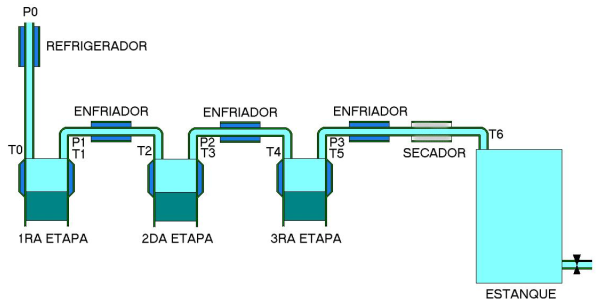
\includegraphics[width = 0.7\linewidth]{Equipo}
\caption{Esquema del equipo del laboratorio}
\label{f:Equipo}
\end{figure}
\section{Metodología}
Para tomar las mediciones se ubican estudiantes en los distintos puntos de medición: en la pantalla que muestra las temperaturas y en los manómetros. Con el uso de un cronómetro se toma el tiempo y se da partida a la máquina. Cada un minuto se da aviso y el equipo toma las medidas de su puesto simultáneamente y se registran. La última medición se realiza en el minuto posterior al sonido de la máquina que indica que se ha llegado a una presión crítica.

\section{Memoria de cálculo}
Mediante el uso de las ecuaciones \ref{e:PavoRaton} y \ref{e:Politropico} se puede deducir que, para una misma masa de aire en dos situaciones distintas (designadas por los subindices 1 y 2), el coeficiente politrópico está dado por la ecuación \ref{e:CoefPoli}

\begin{equation}
n = \frac{1}
{1-\frac{\ln(T_2/T_1)}{\ln(P_2/P_1)}}
\label{e:CoefPoli}
\end{equation}

Para determinar el volumen que se toma en cada instante se utiliza la ecuación \ref{e:PavoRaton} tanto al exterior como en el estanque luego de la compresión y se tiene la relación:
\begin{equation}
V_{0} = V_{\text{est}} \frac{P_3}{T_6} \frac{T_0}{P_0}
\label{e:Volumen}
\end{equation}

Con la ecuación \ref{e:Volumen} se puede determinar también el caudal $\dot{V_0}$ derivando con respecto al tiempo como se hace a continuación:

\begin{equation}
\dot{V_0} = V_{\text{est}}\dot{
\left( \frac{P_3}{T_6} 
\frac{T_0}{P_0}
\right)}
\label{e:Caudal}
\end{equation} 

Por ultimo se puede deteminar el volumen en cada punto mediante la ecuación \ref{e:PavoRaton} de manera que:

\begin{equation}
V_i = V_{\text{est}} \frac{P_3}{T_6} \frac{T_i}{P_i}
\end{equation}
\newpage
\section{Resultados}

Las figuras \ref{f:Temperatura} y \ref{f:Presion} muestran la evolución de la temperatura y presión en cada punto de medición respectivamente.

\begin{figure}[H]
\begin{minipage}{0.5\linewidth}
\centering
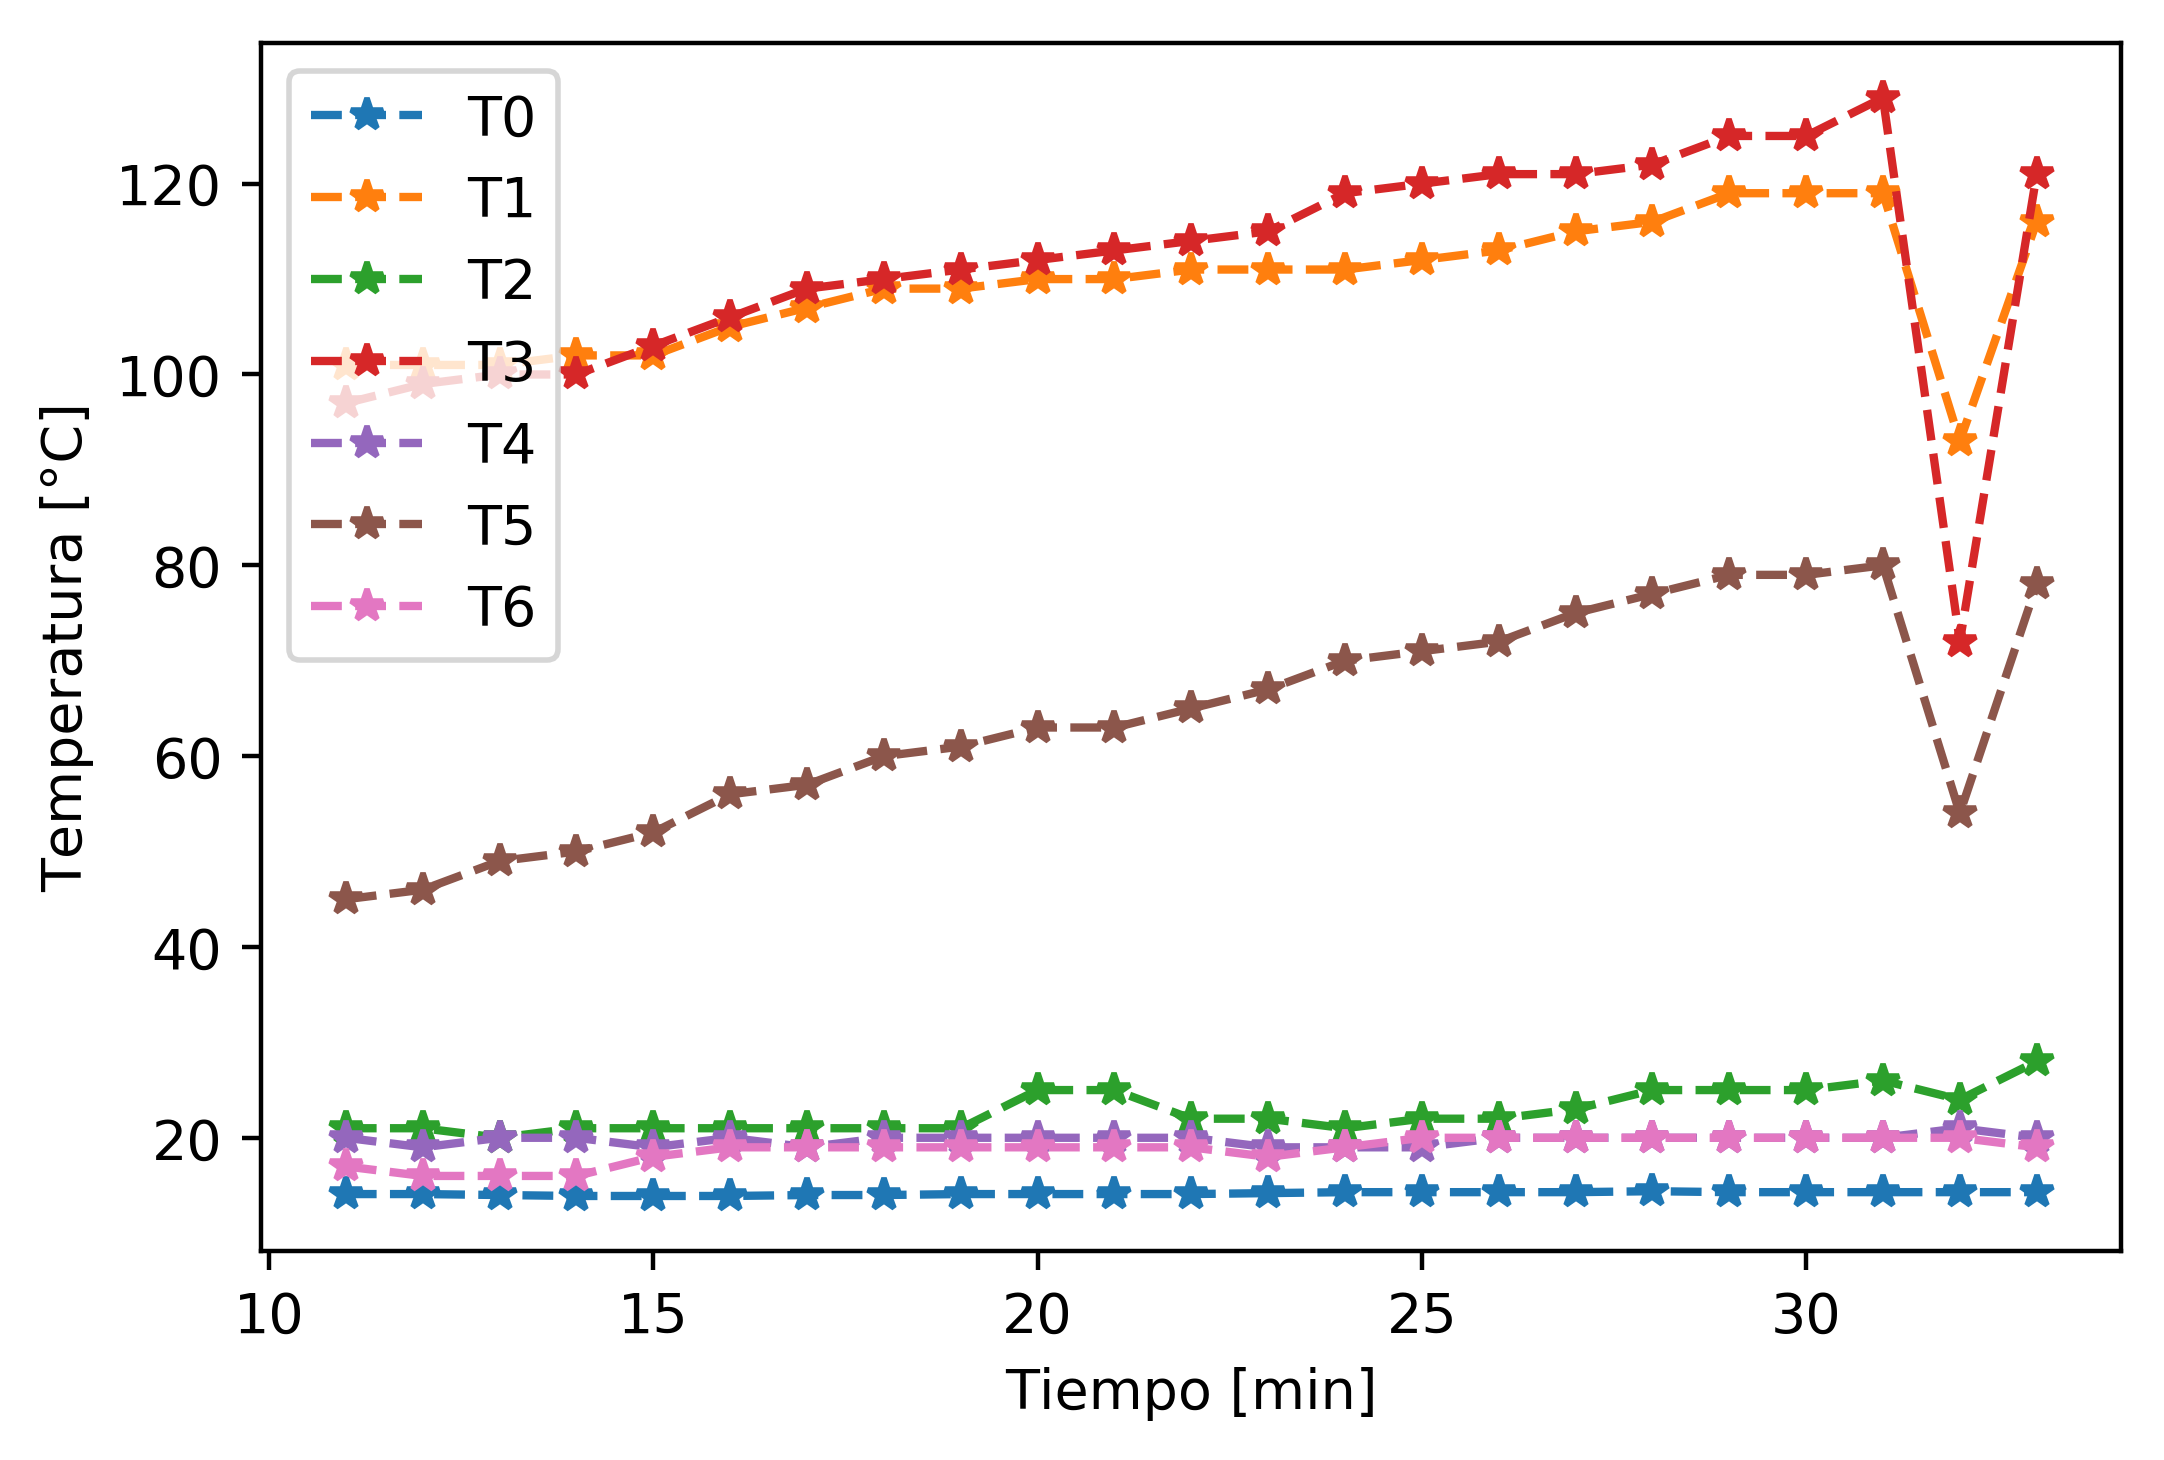
\includegraphics[width = \linewidth]{Temperatura}
\caption{Temperaturas medidas en el tiempo.}
\label{f:Temperatura}
\end{minipage}
\begin{minipage}{0.5\linewidth}
\centering
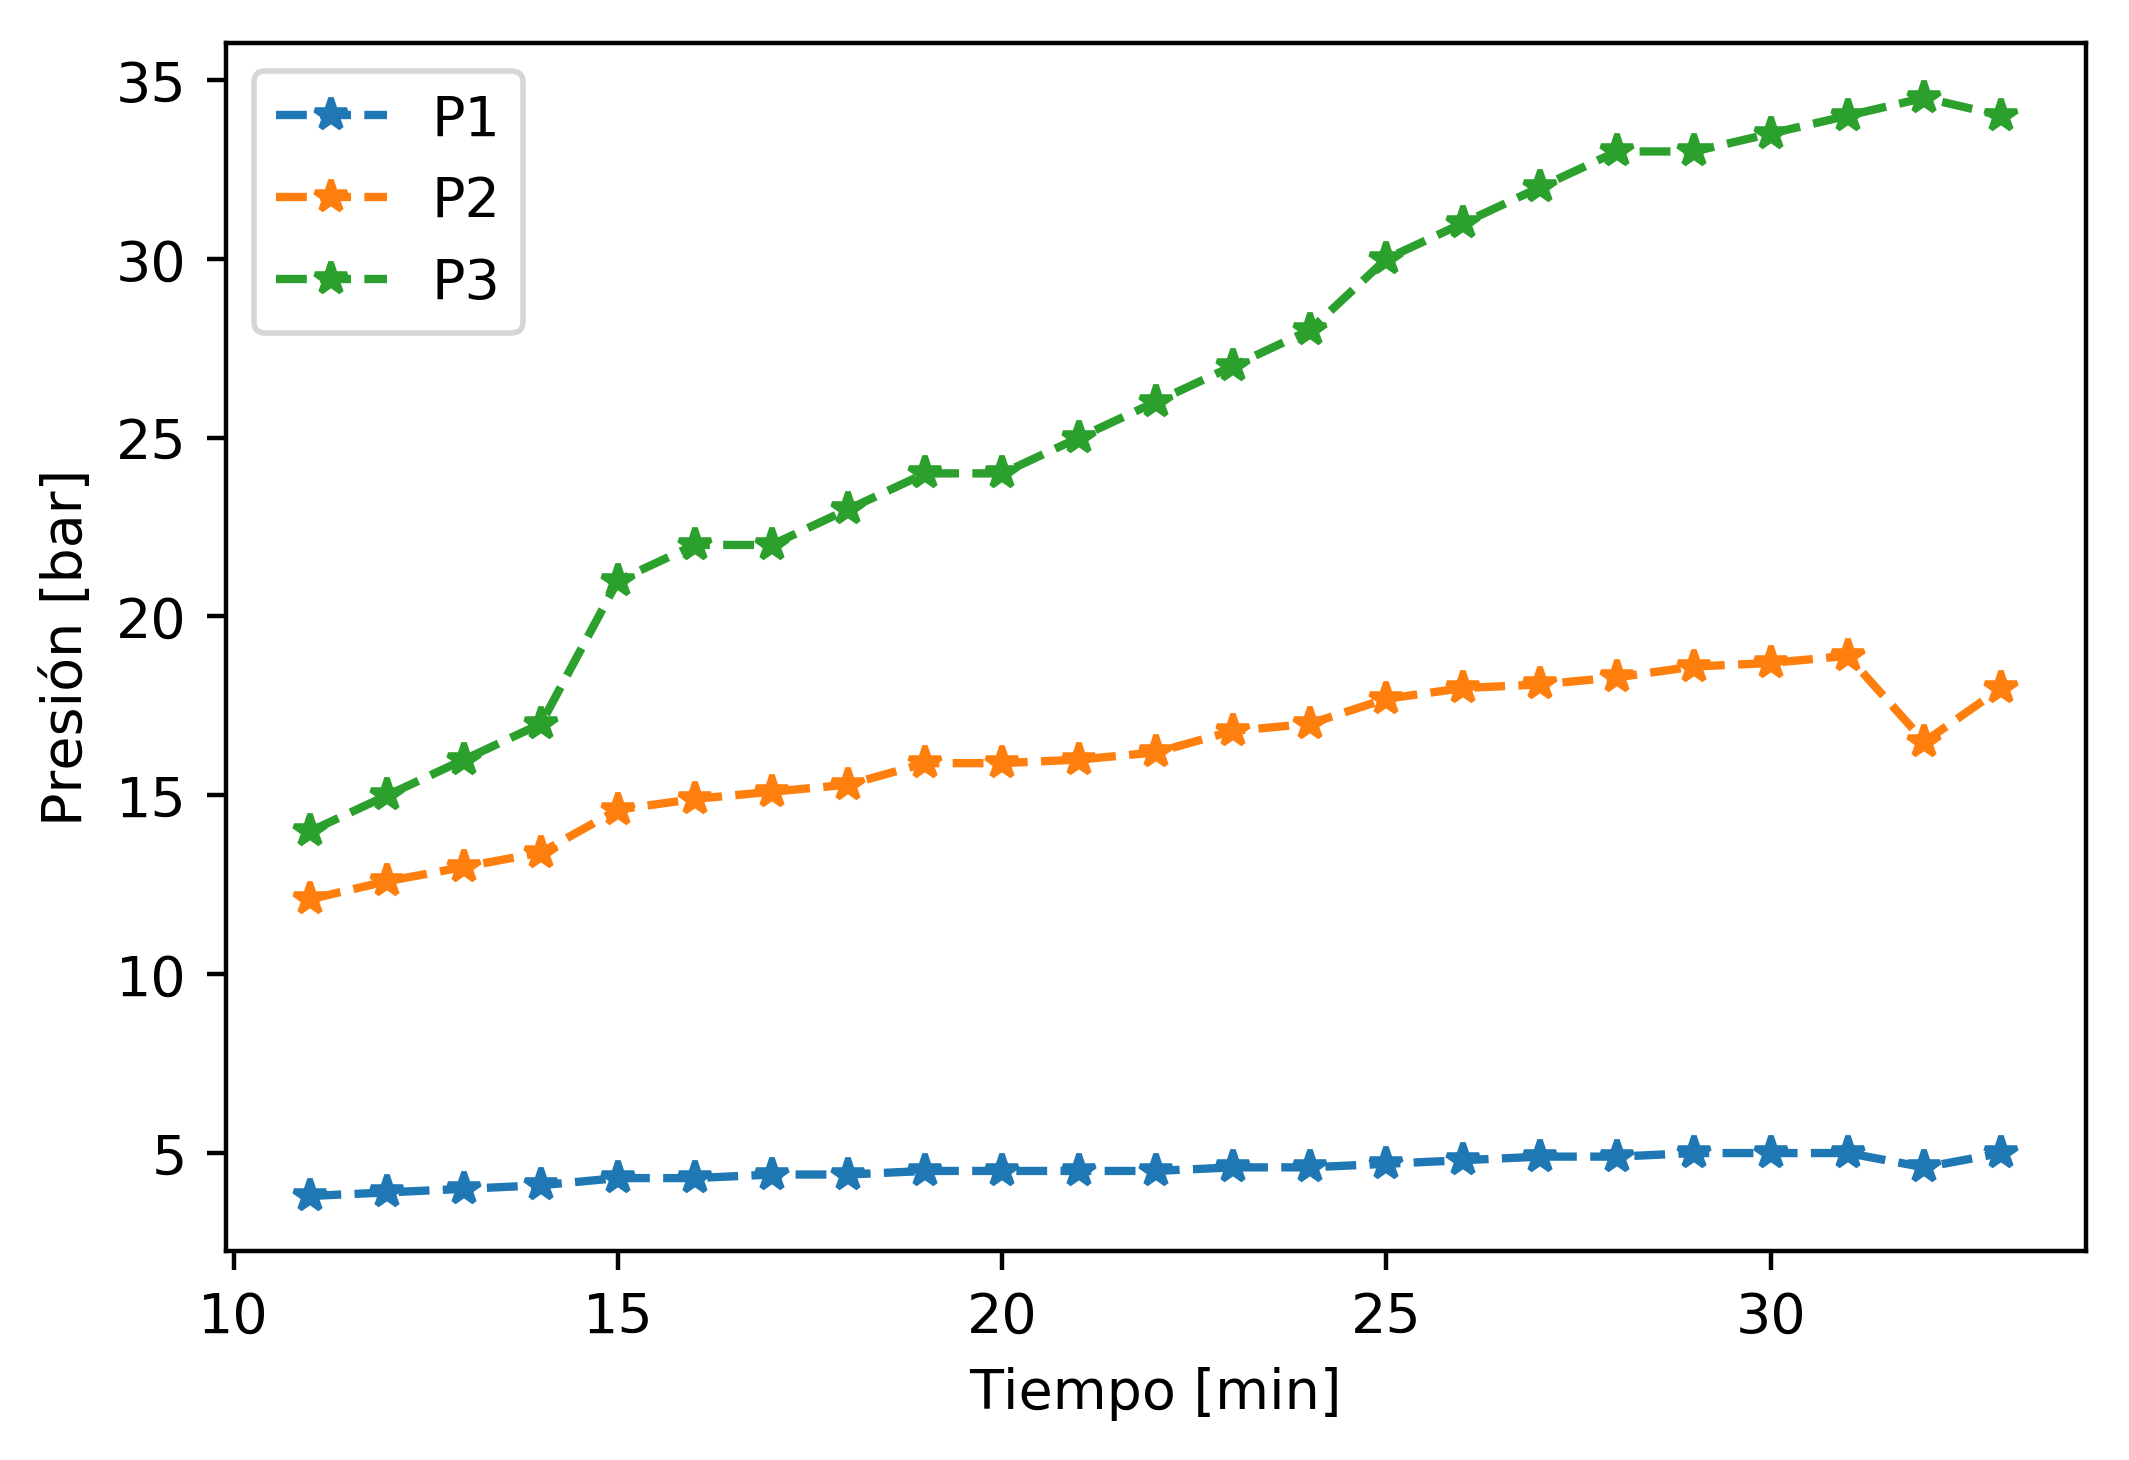
\includegraphics[width = \linewidth]{Presiones}
\caption{Presiones medidas en el tiempo.}
\label{f:Presion}
\end{minipage}
\end{figure}


En la figura \ref{f:Coeficiente} se muestra el coeficiente calculado con la ecuación \ref{e:CoefPoli} para el cada compresor a en cada instante de tiempo. 
\begin{figure}[H]
\centering
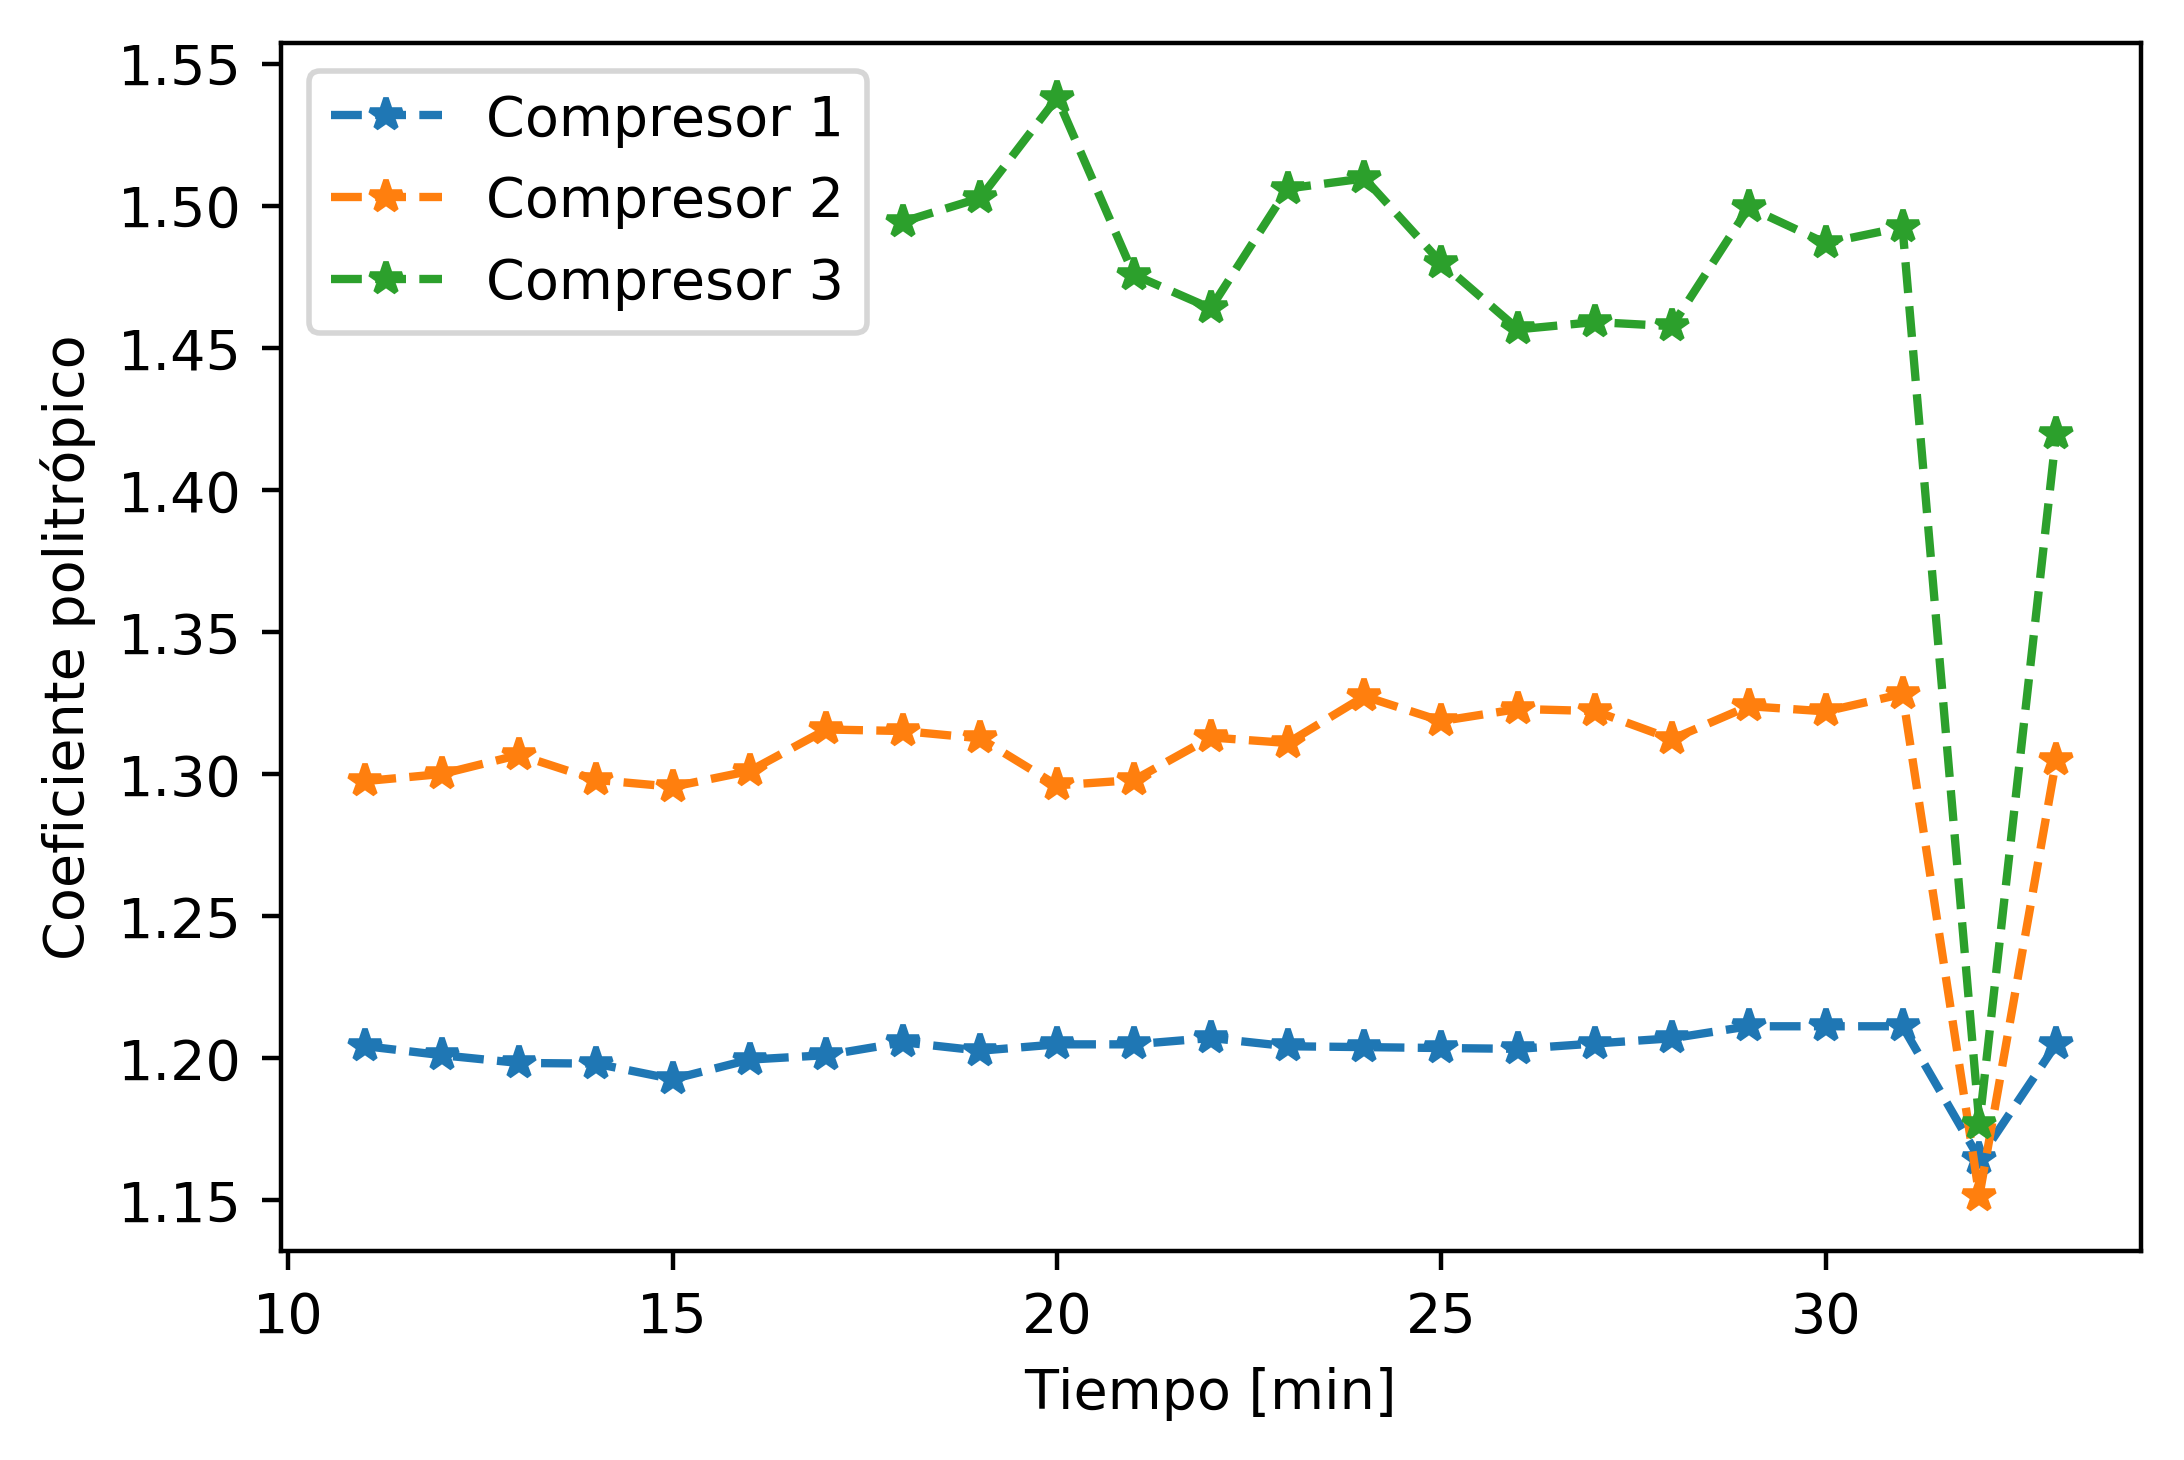
\includegraphics[width=0.6\linewidth]{Coef}
\caption{Coeficiente politrópico en los distintos compresores.}
\label{f:Coeficiente}
\end{figure}


En las figuras \ref{f:CTiempo} y \ref{f:CPresion} se muestran los caudales en función de los parámetros tiempo y presión de descarga calculados con la ecuación\ref{e:Caudal}. Mientras que las figuras \ref{f:t14} a \ref{f:t33} muestran los diagramas \textit{Pv} en distintos instantes de tiempos y fueron calculados con la ecuación \ref{e:Volumen}.

\begin{figure}[H]
\begin{minipage}{0.5\linewidth}
\centering
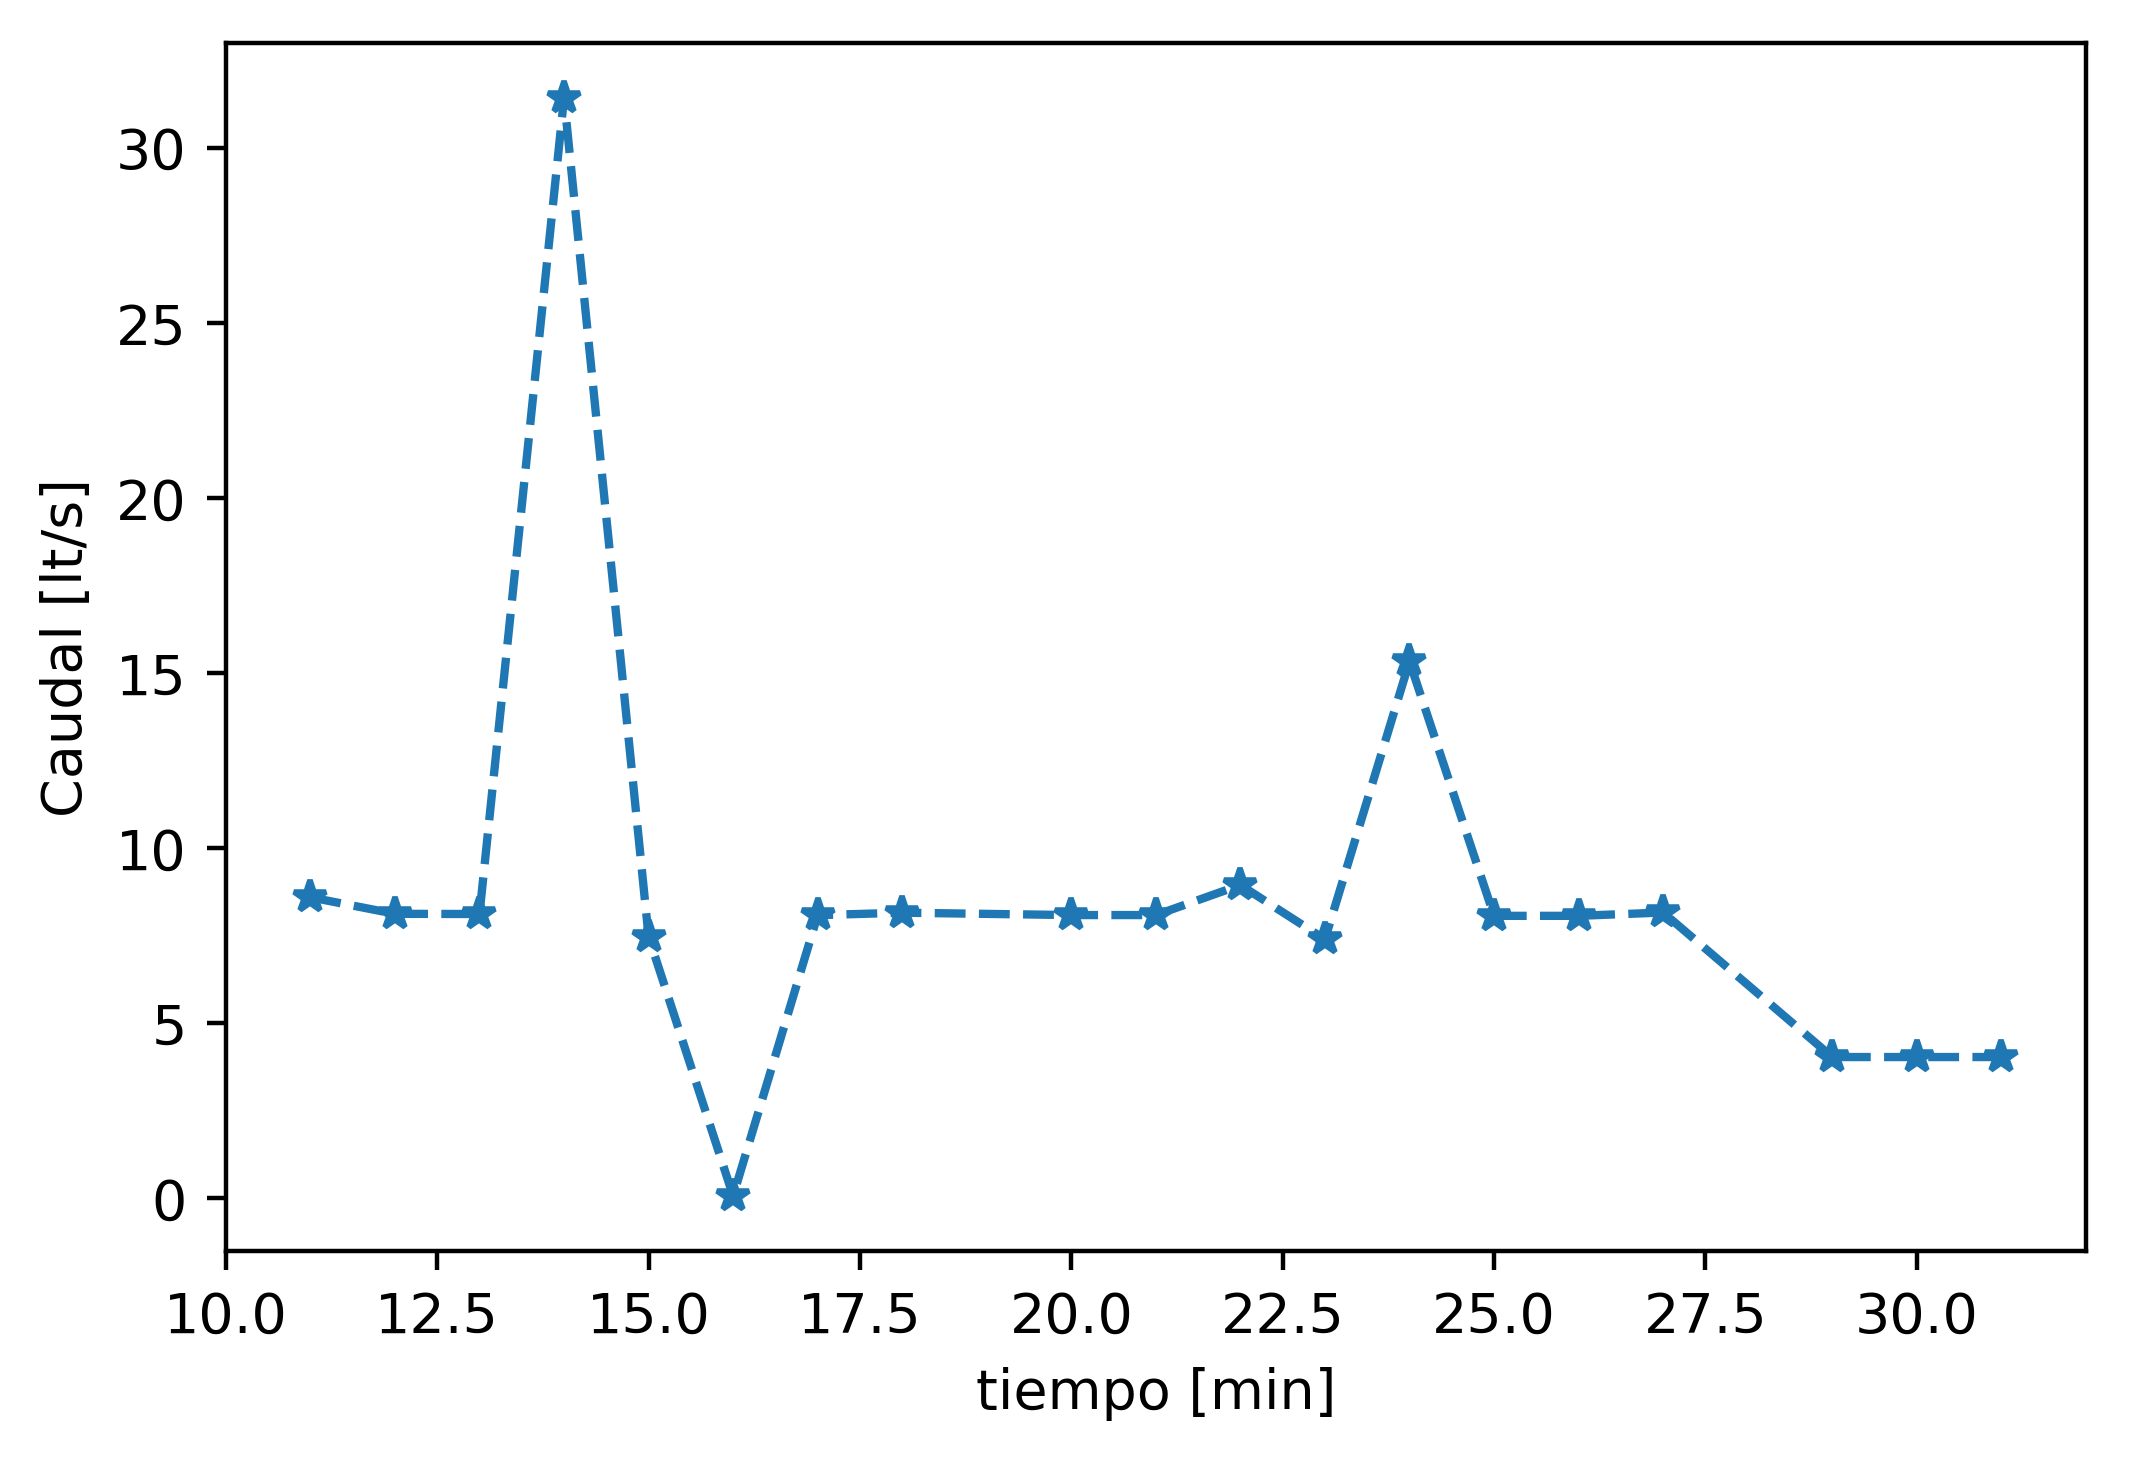
\includegraphics[width = \linewidth]{CaudalTiempo}
\caption{Caudal de entrada calculado en el tiempo.}
\label{f:CTiempo}
\end{minipage}
\begin{minipage}{0.5\linewidth}
\centering
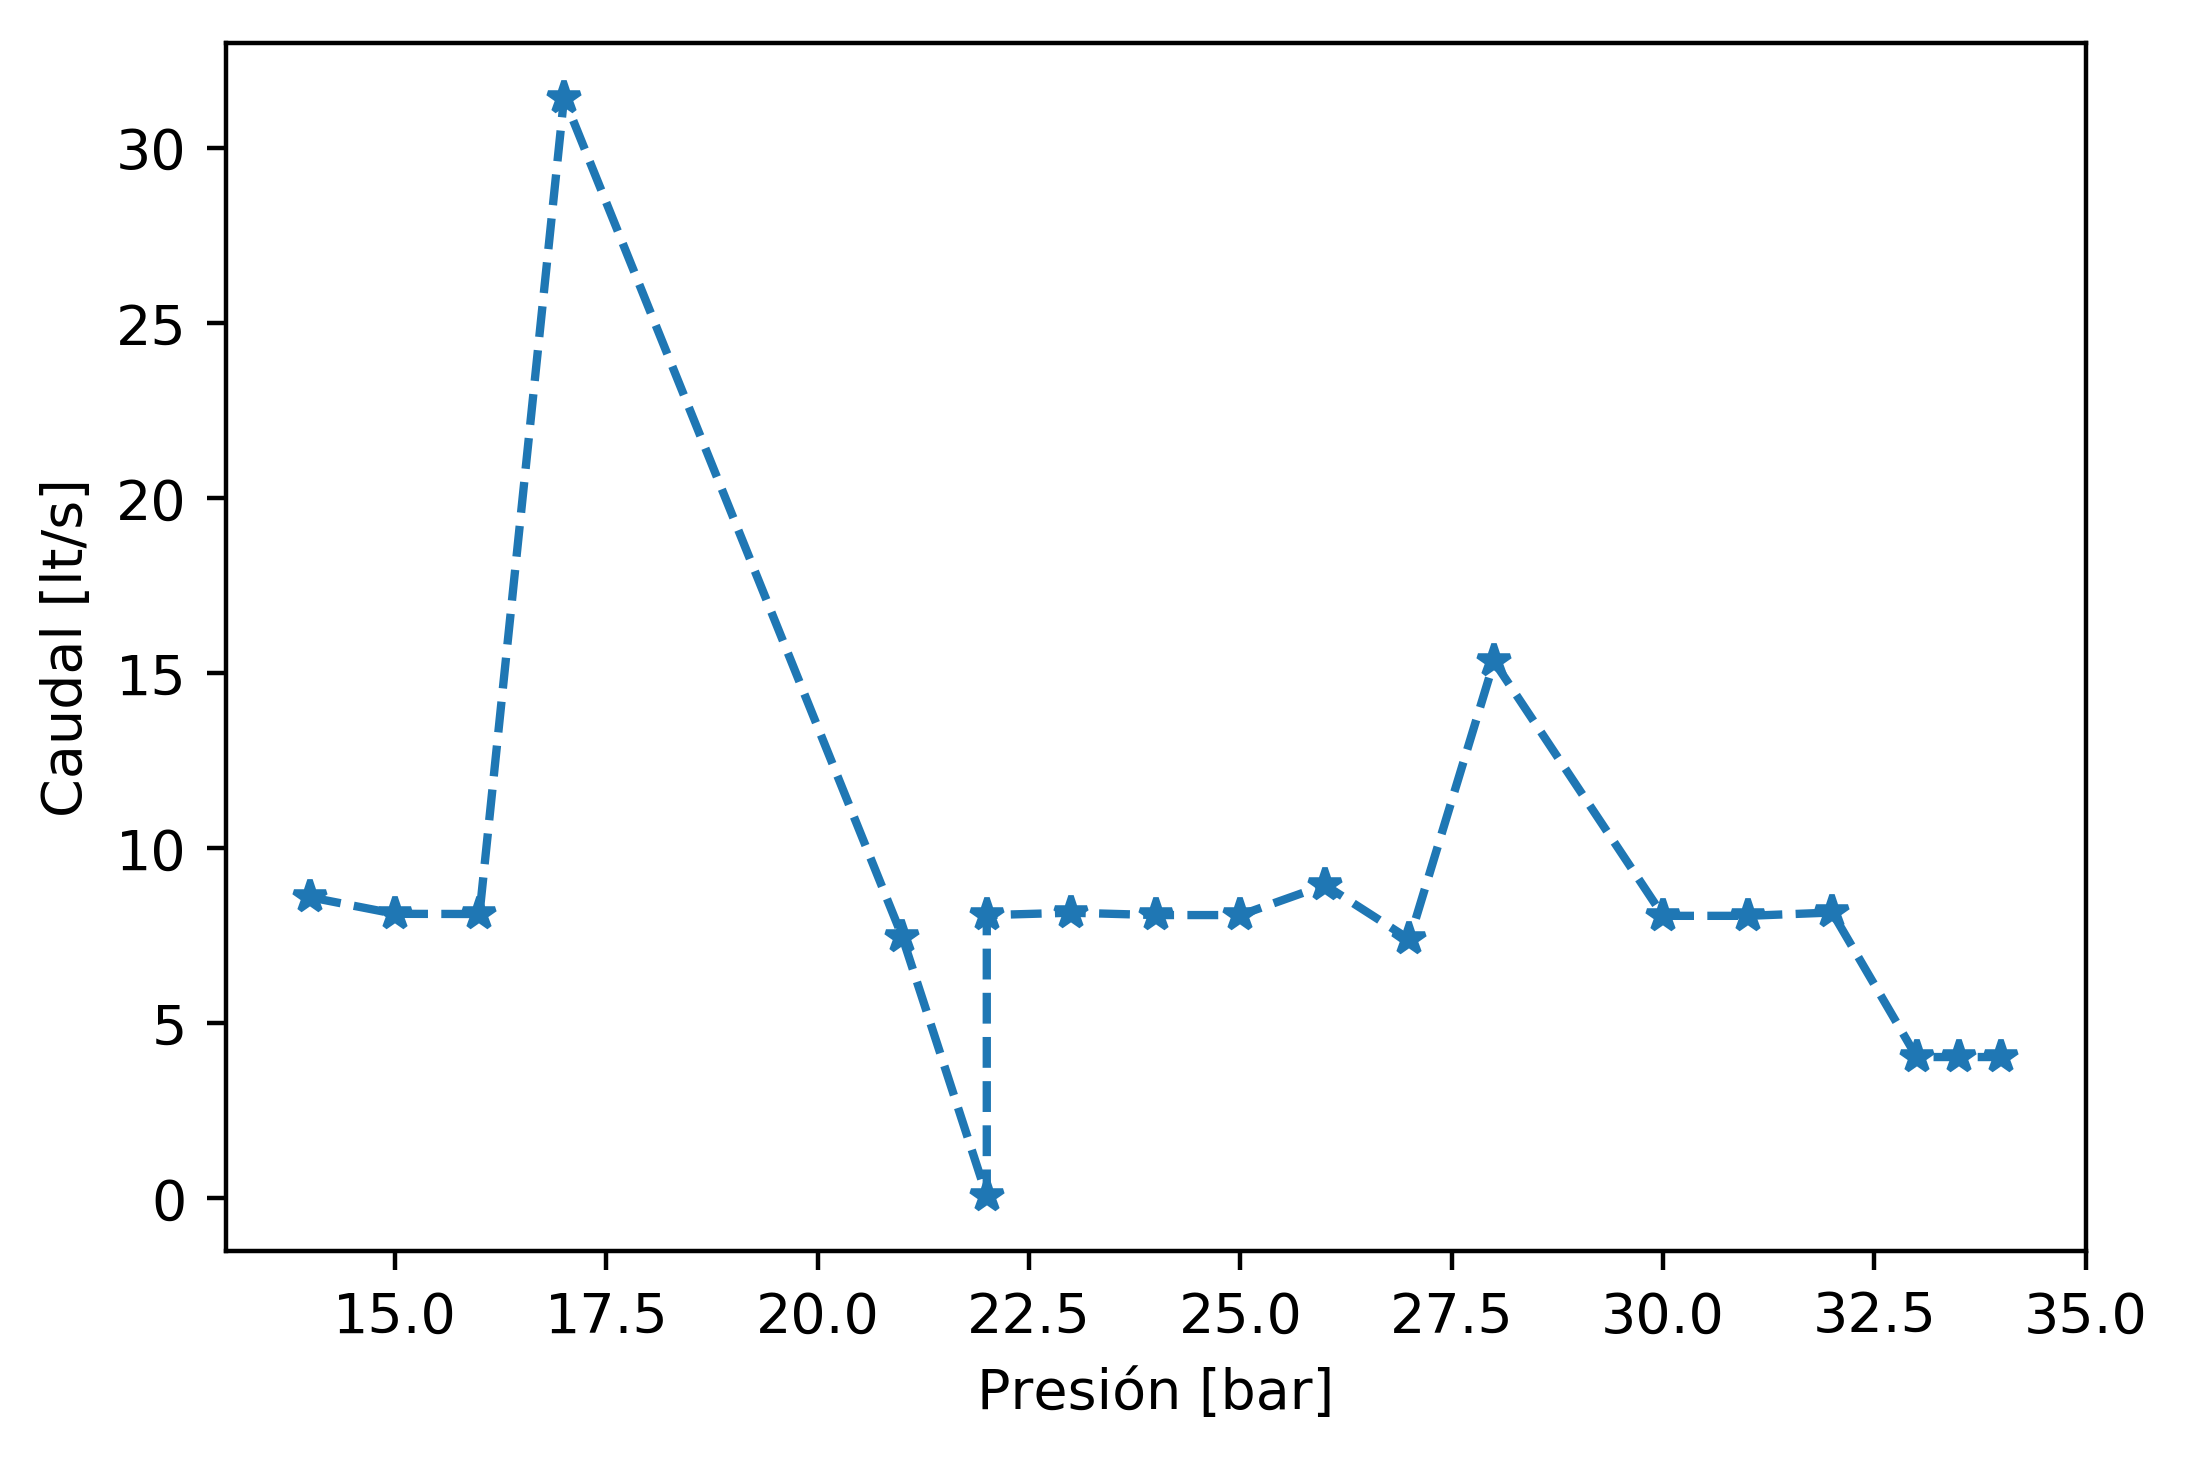
\includegraphics[width = \linewidth]{CaudalPresion}
\caption{Caudal para cada presión de descarga.}
\label{f:CPresion}
\end{minipage}
\end{figure}

\begin{figure}[H]
\centering
\begin{minipage}{0.49\linewidth}
\centering
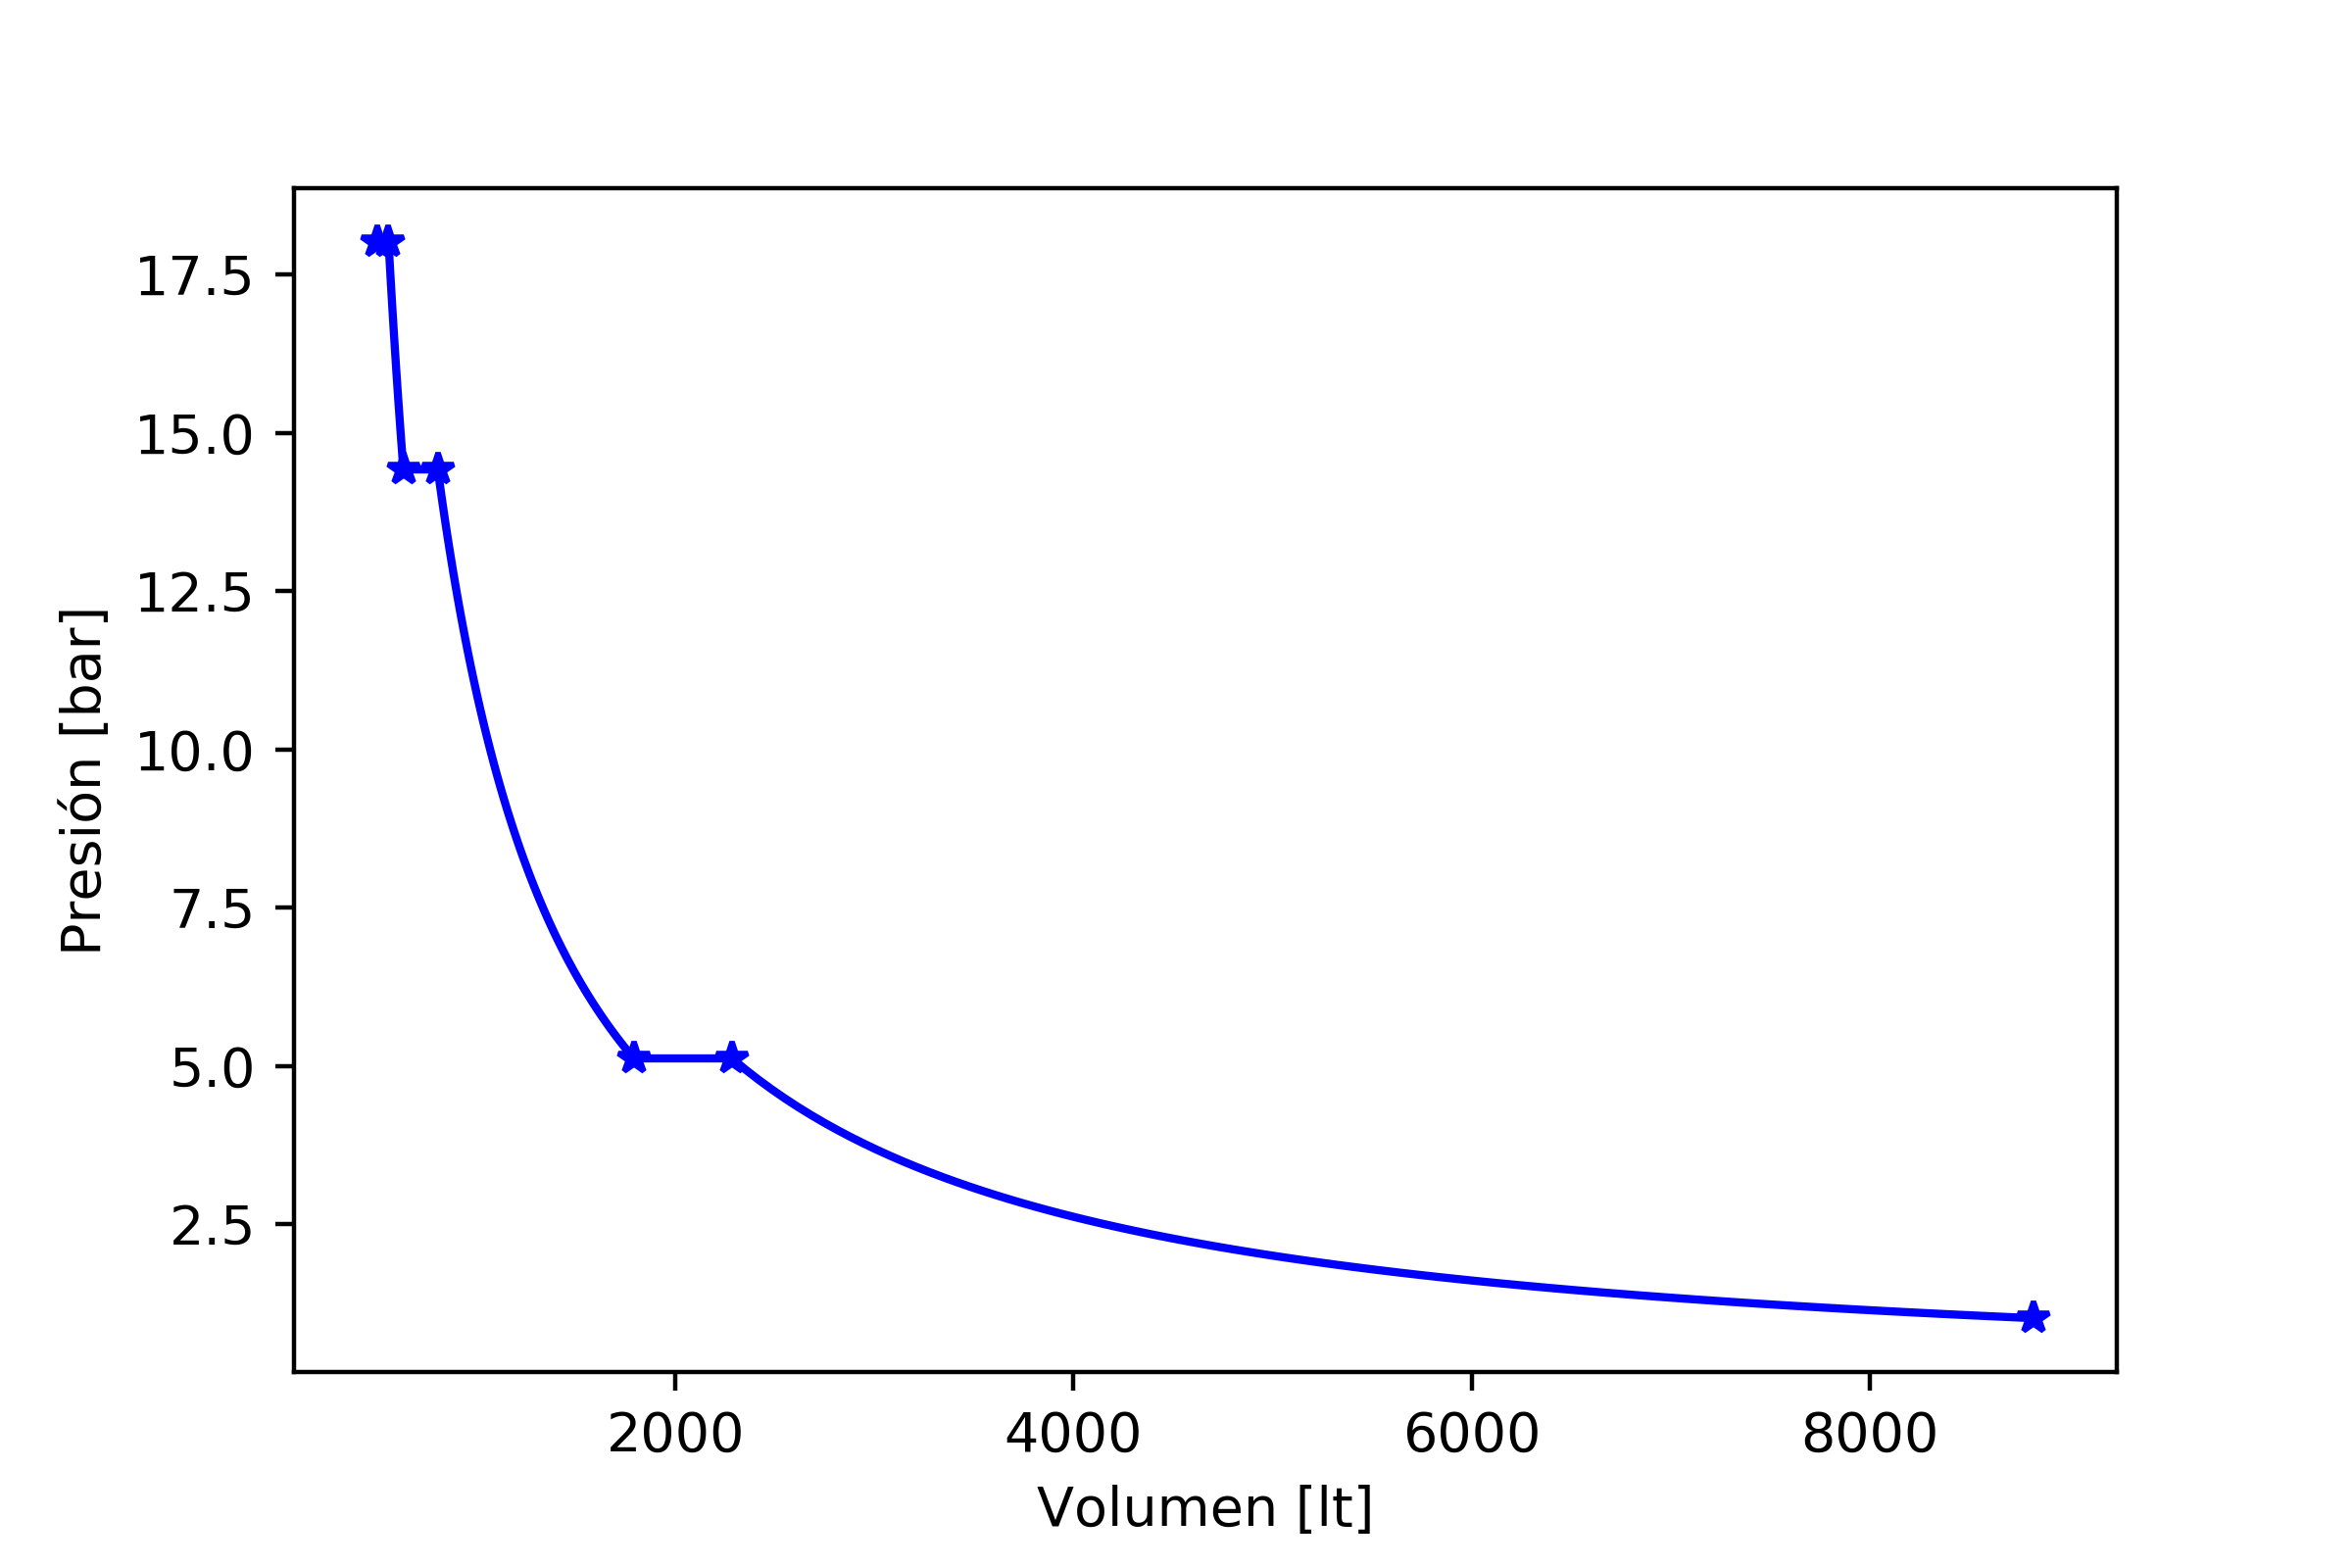
\includegraphics[width = \linewidth]{tiempo14}
\caption{Diagrama PV para un tiempo de 14[min]}
\label{f:t14}
\end{minipage}
\hfill
\begin{minipage}{0.49\linewidth}
\centering
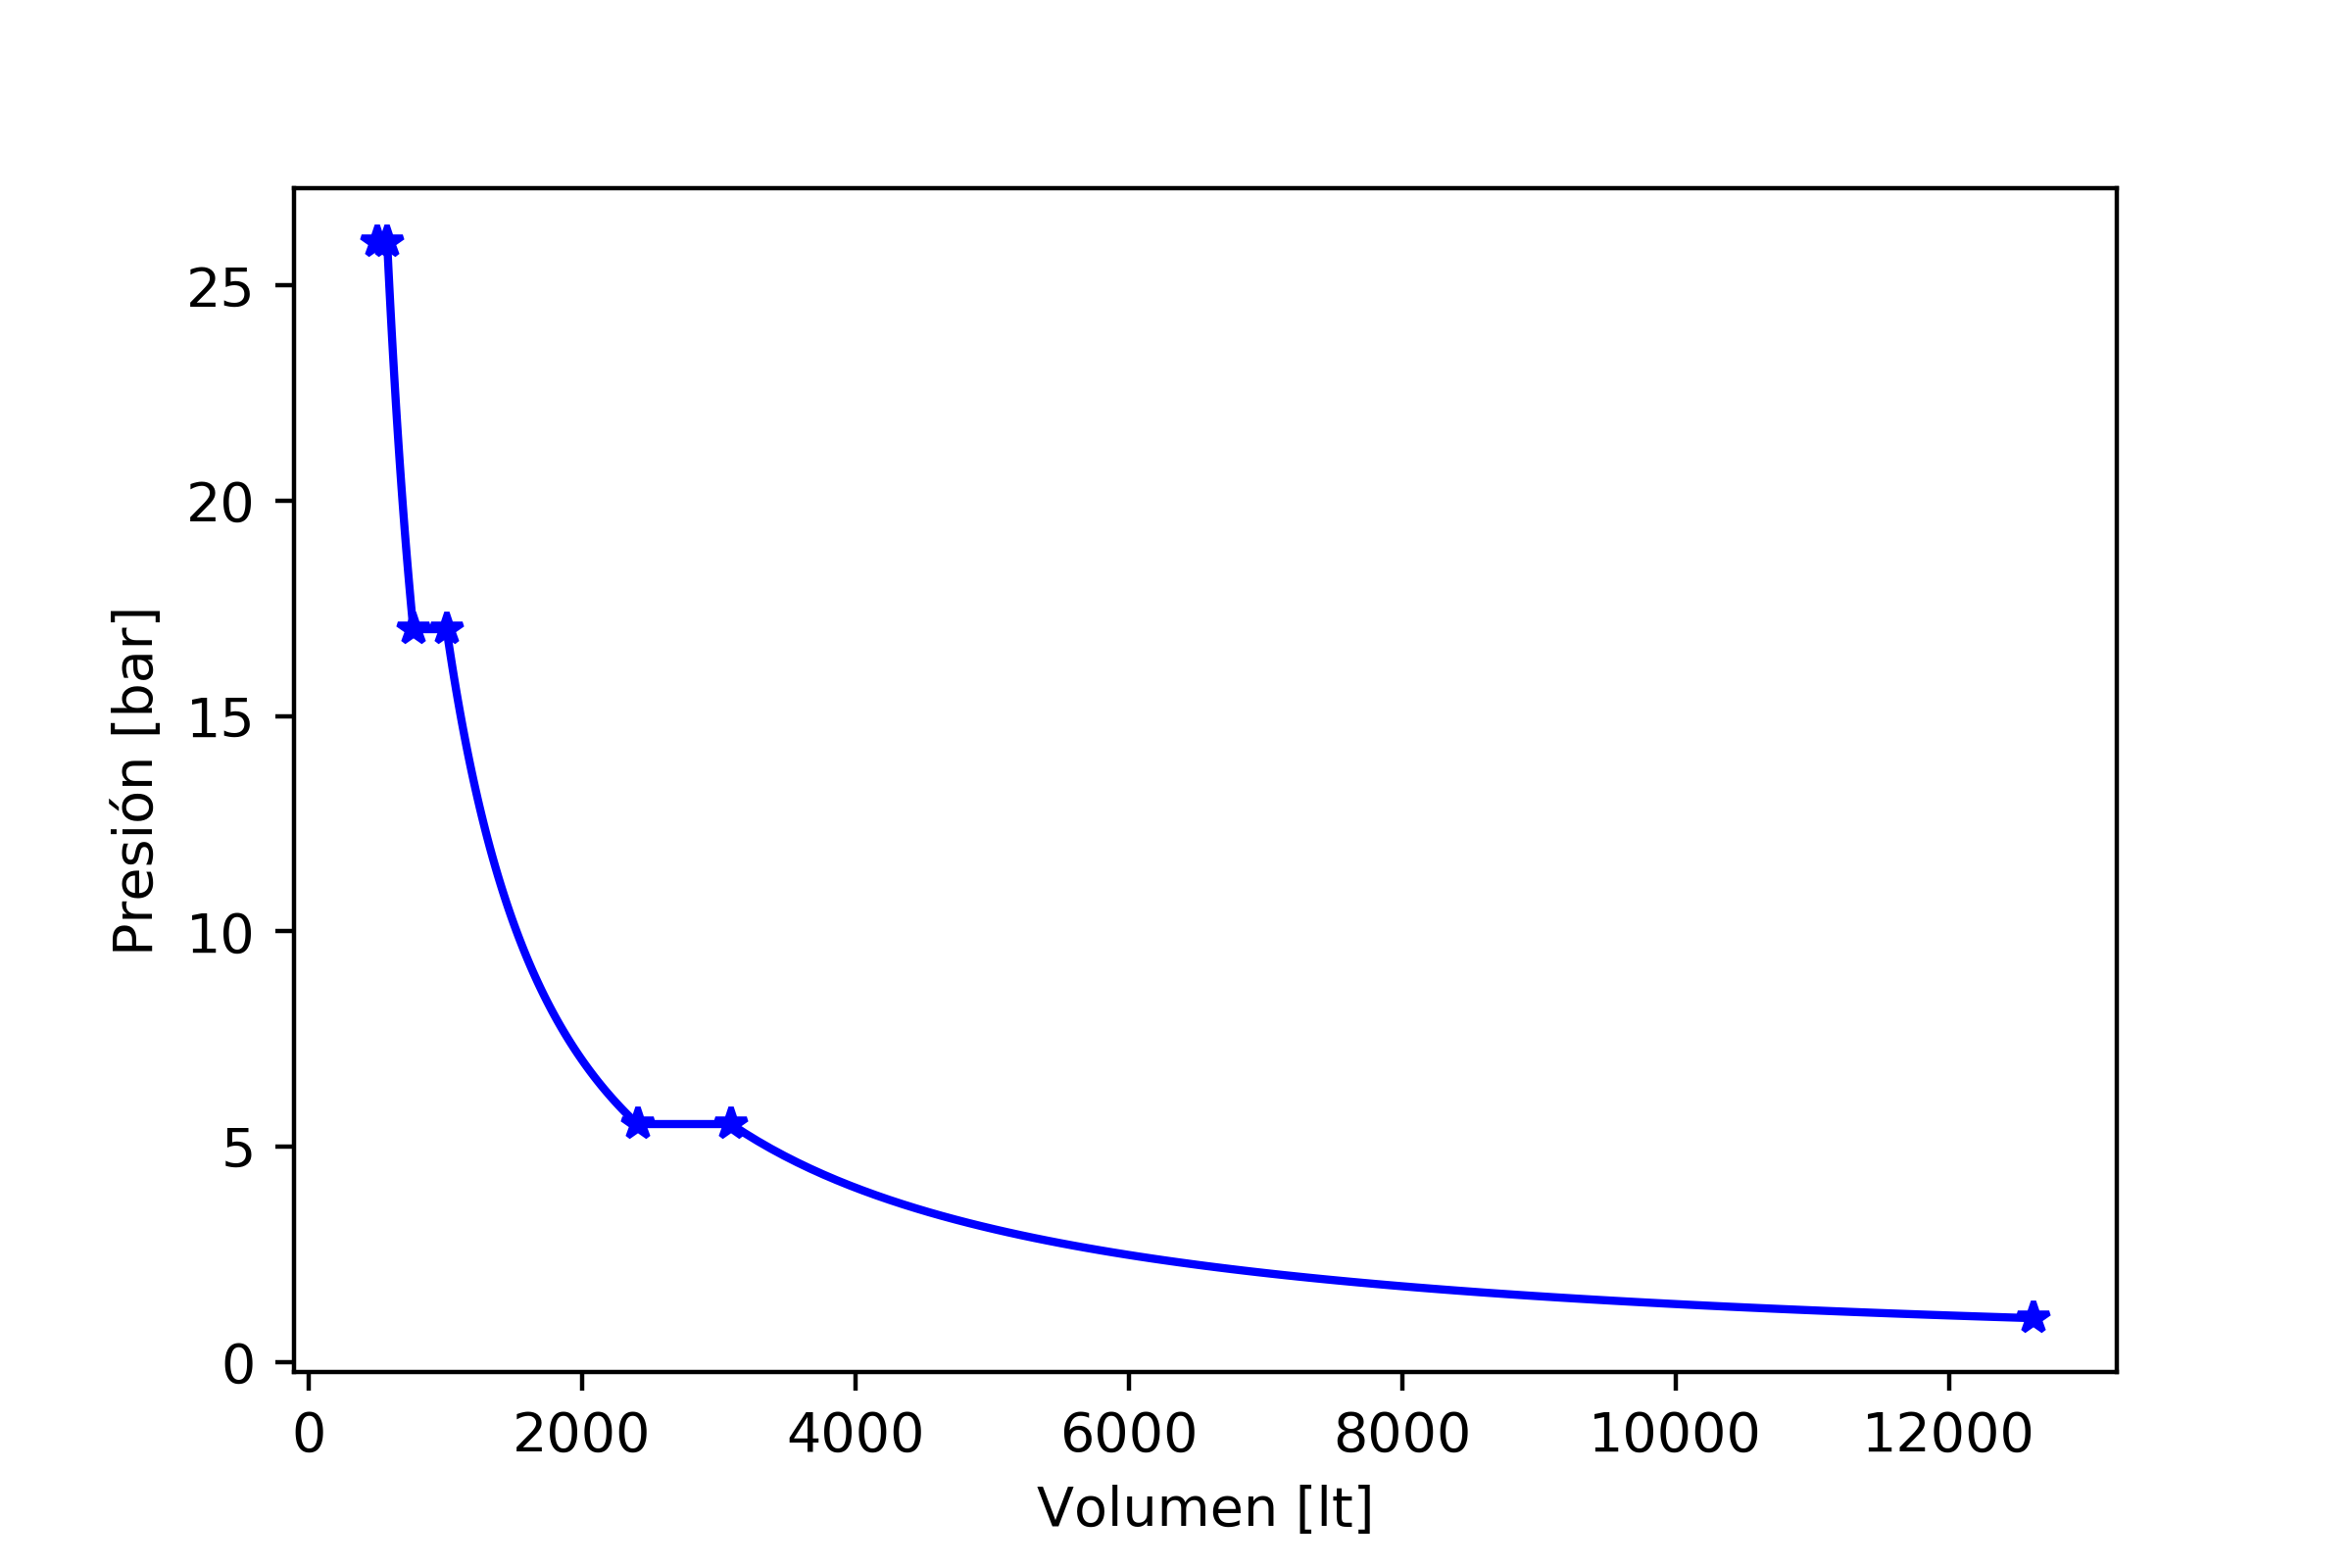
\includegraphics[width = \linewidth]{tiempo21}
\caption{Diagrama PV para un tiempo de 21[min]}
\label{f:t21}
\end{minipage}
\end{figure}

\begin{figure}[H]
\centering
\begin{minipage}{0.49\linewidth}
\centering
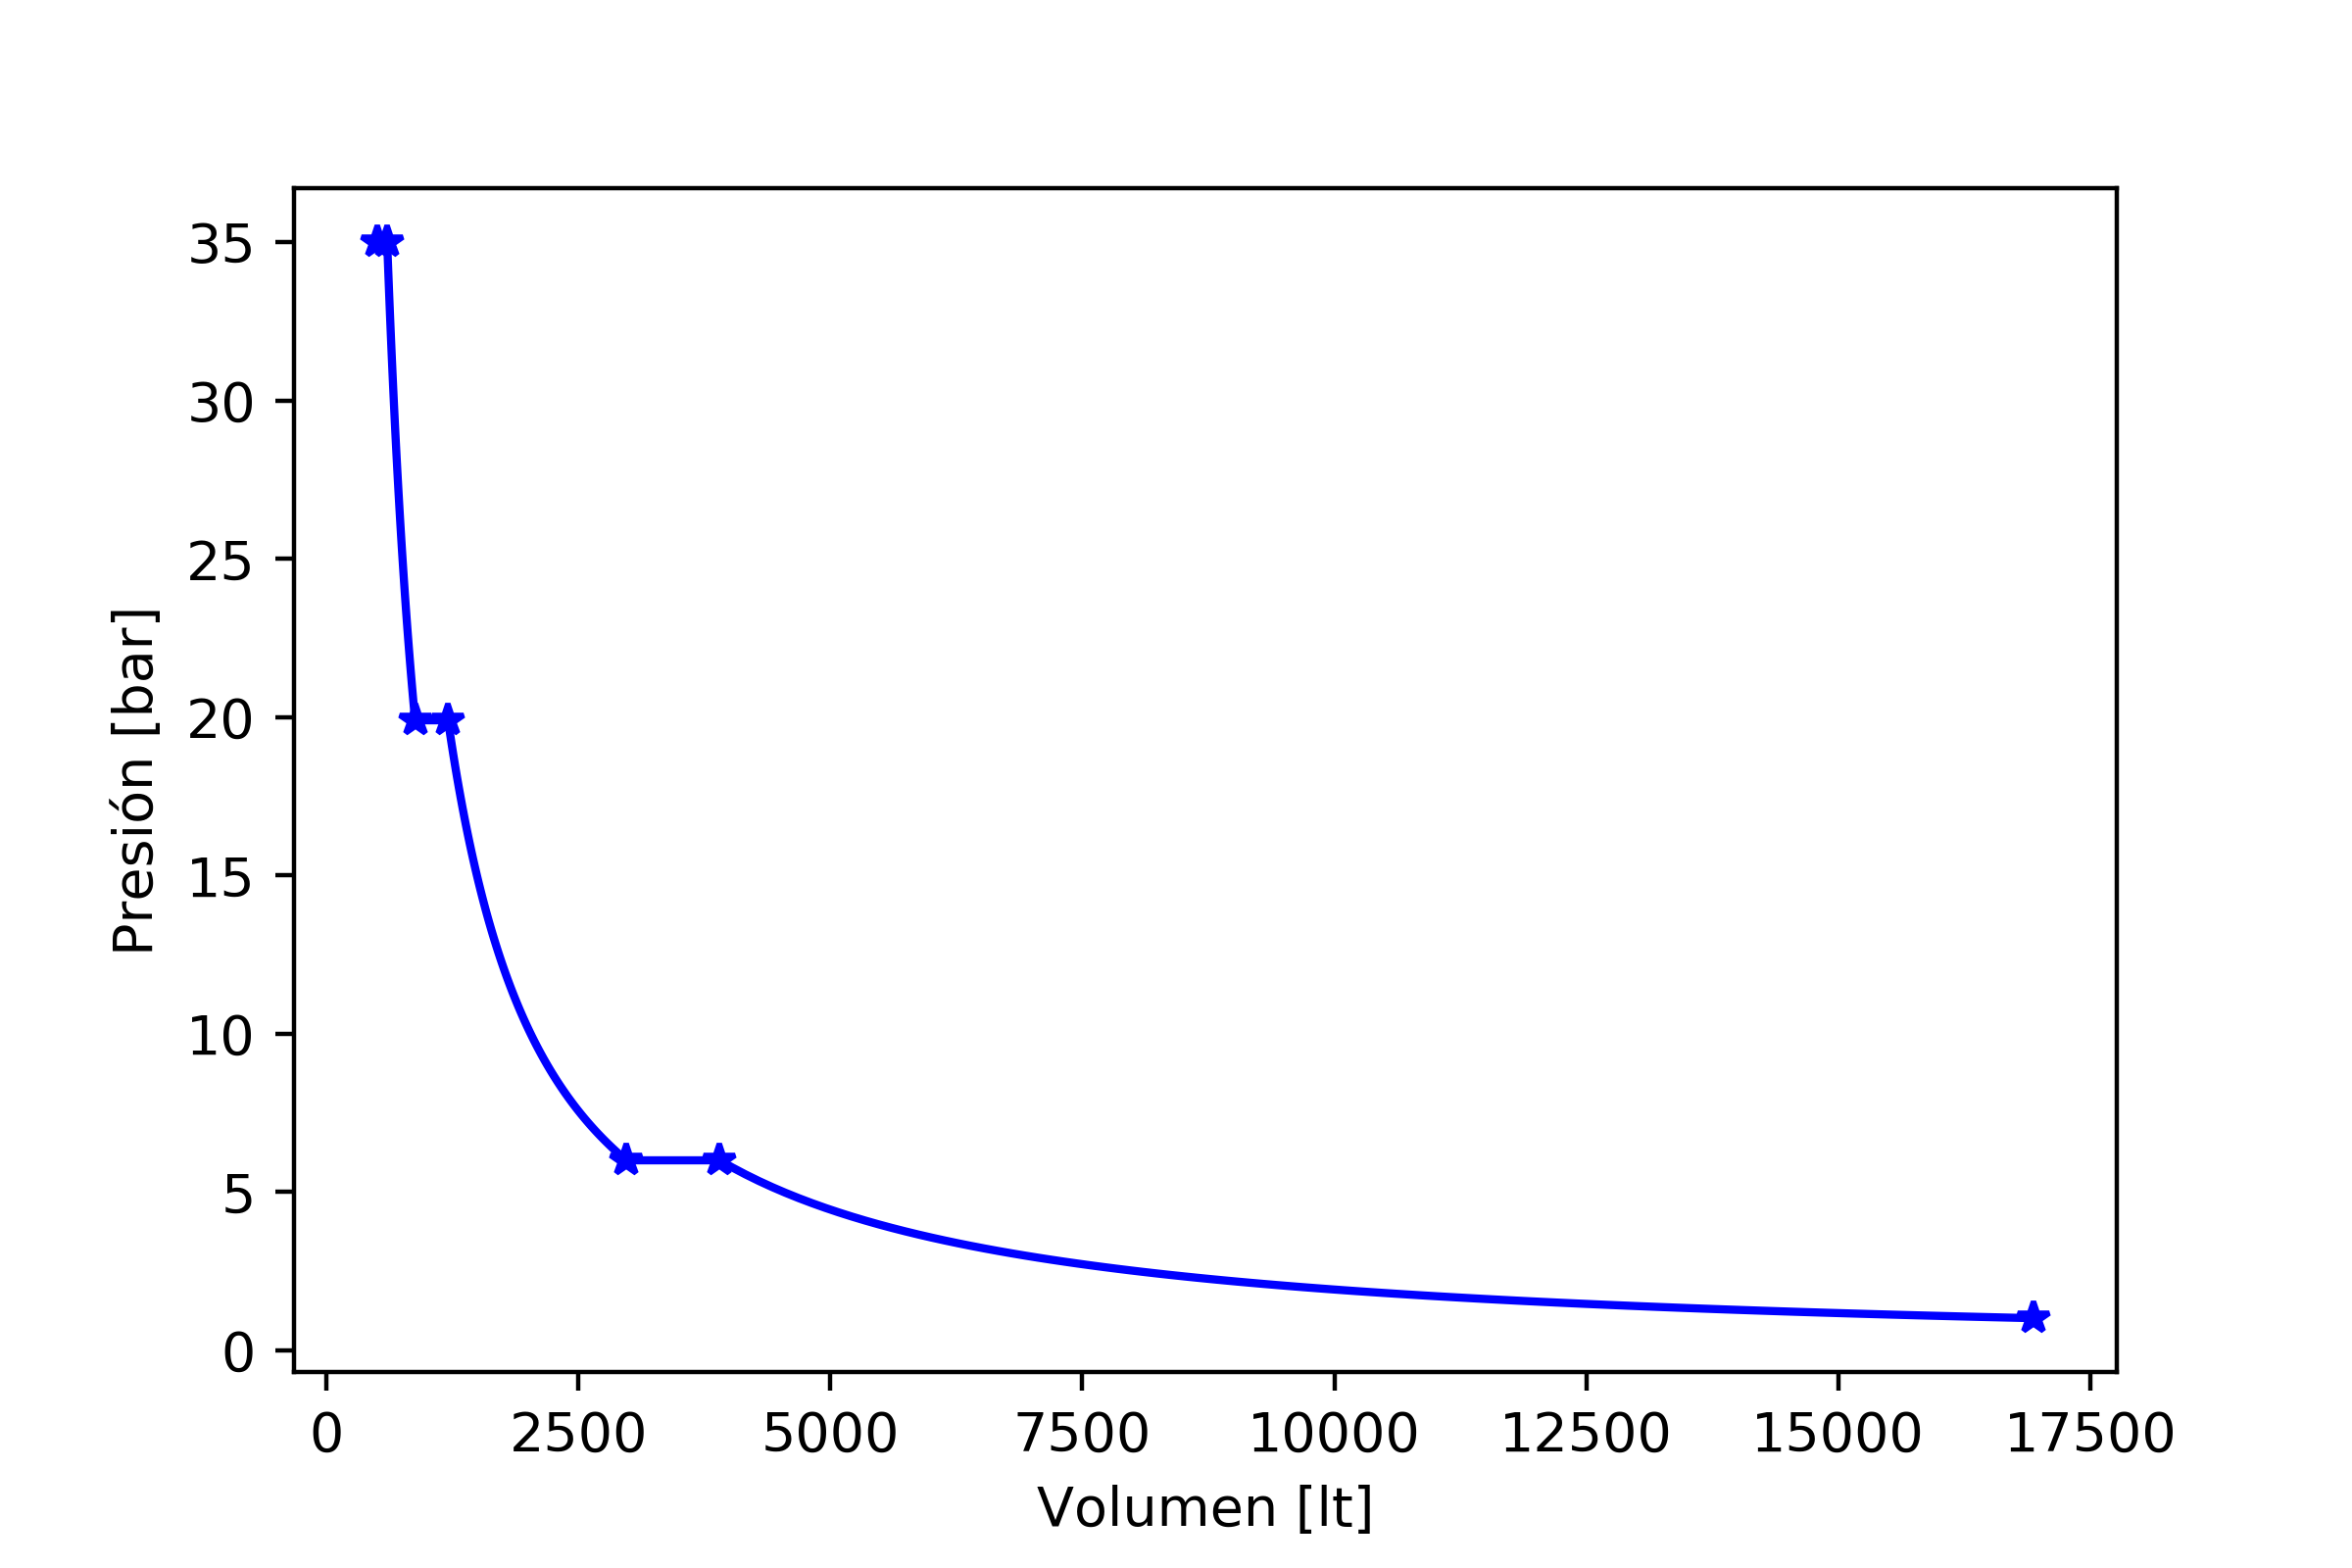
\includegraphics[width = \linewidth]{tiempo31}
\caption{Diagrama PV para un tiempo de 31[min]}
\label{f:t31}
\end{minipage}
\hfill
\begin{minipage}{0.49\linewidth}
\centering
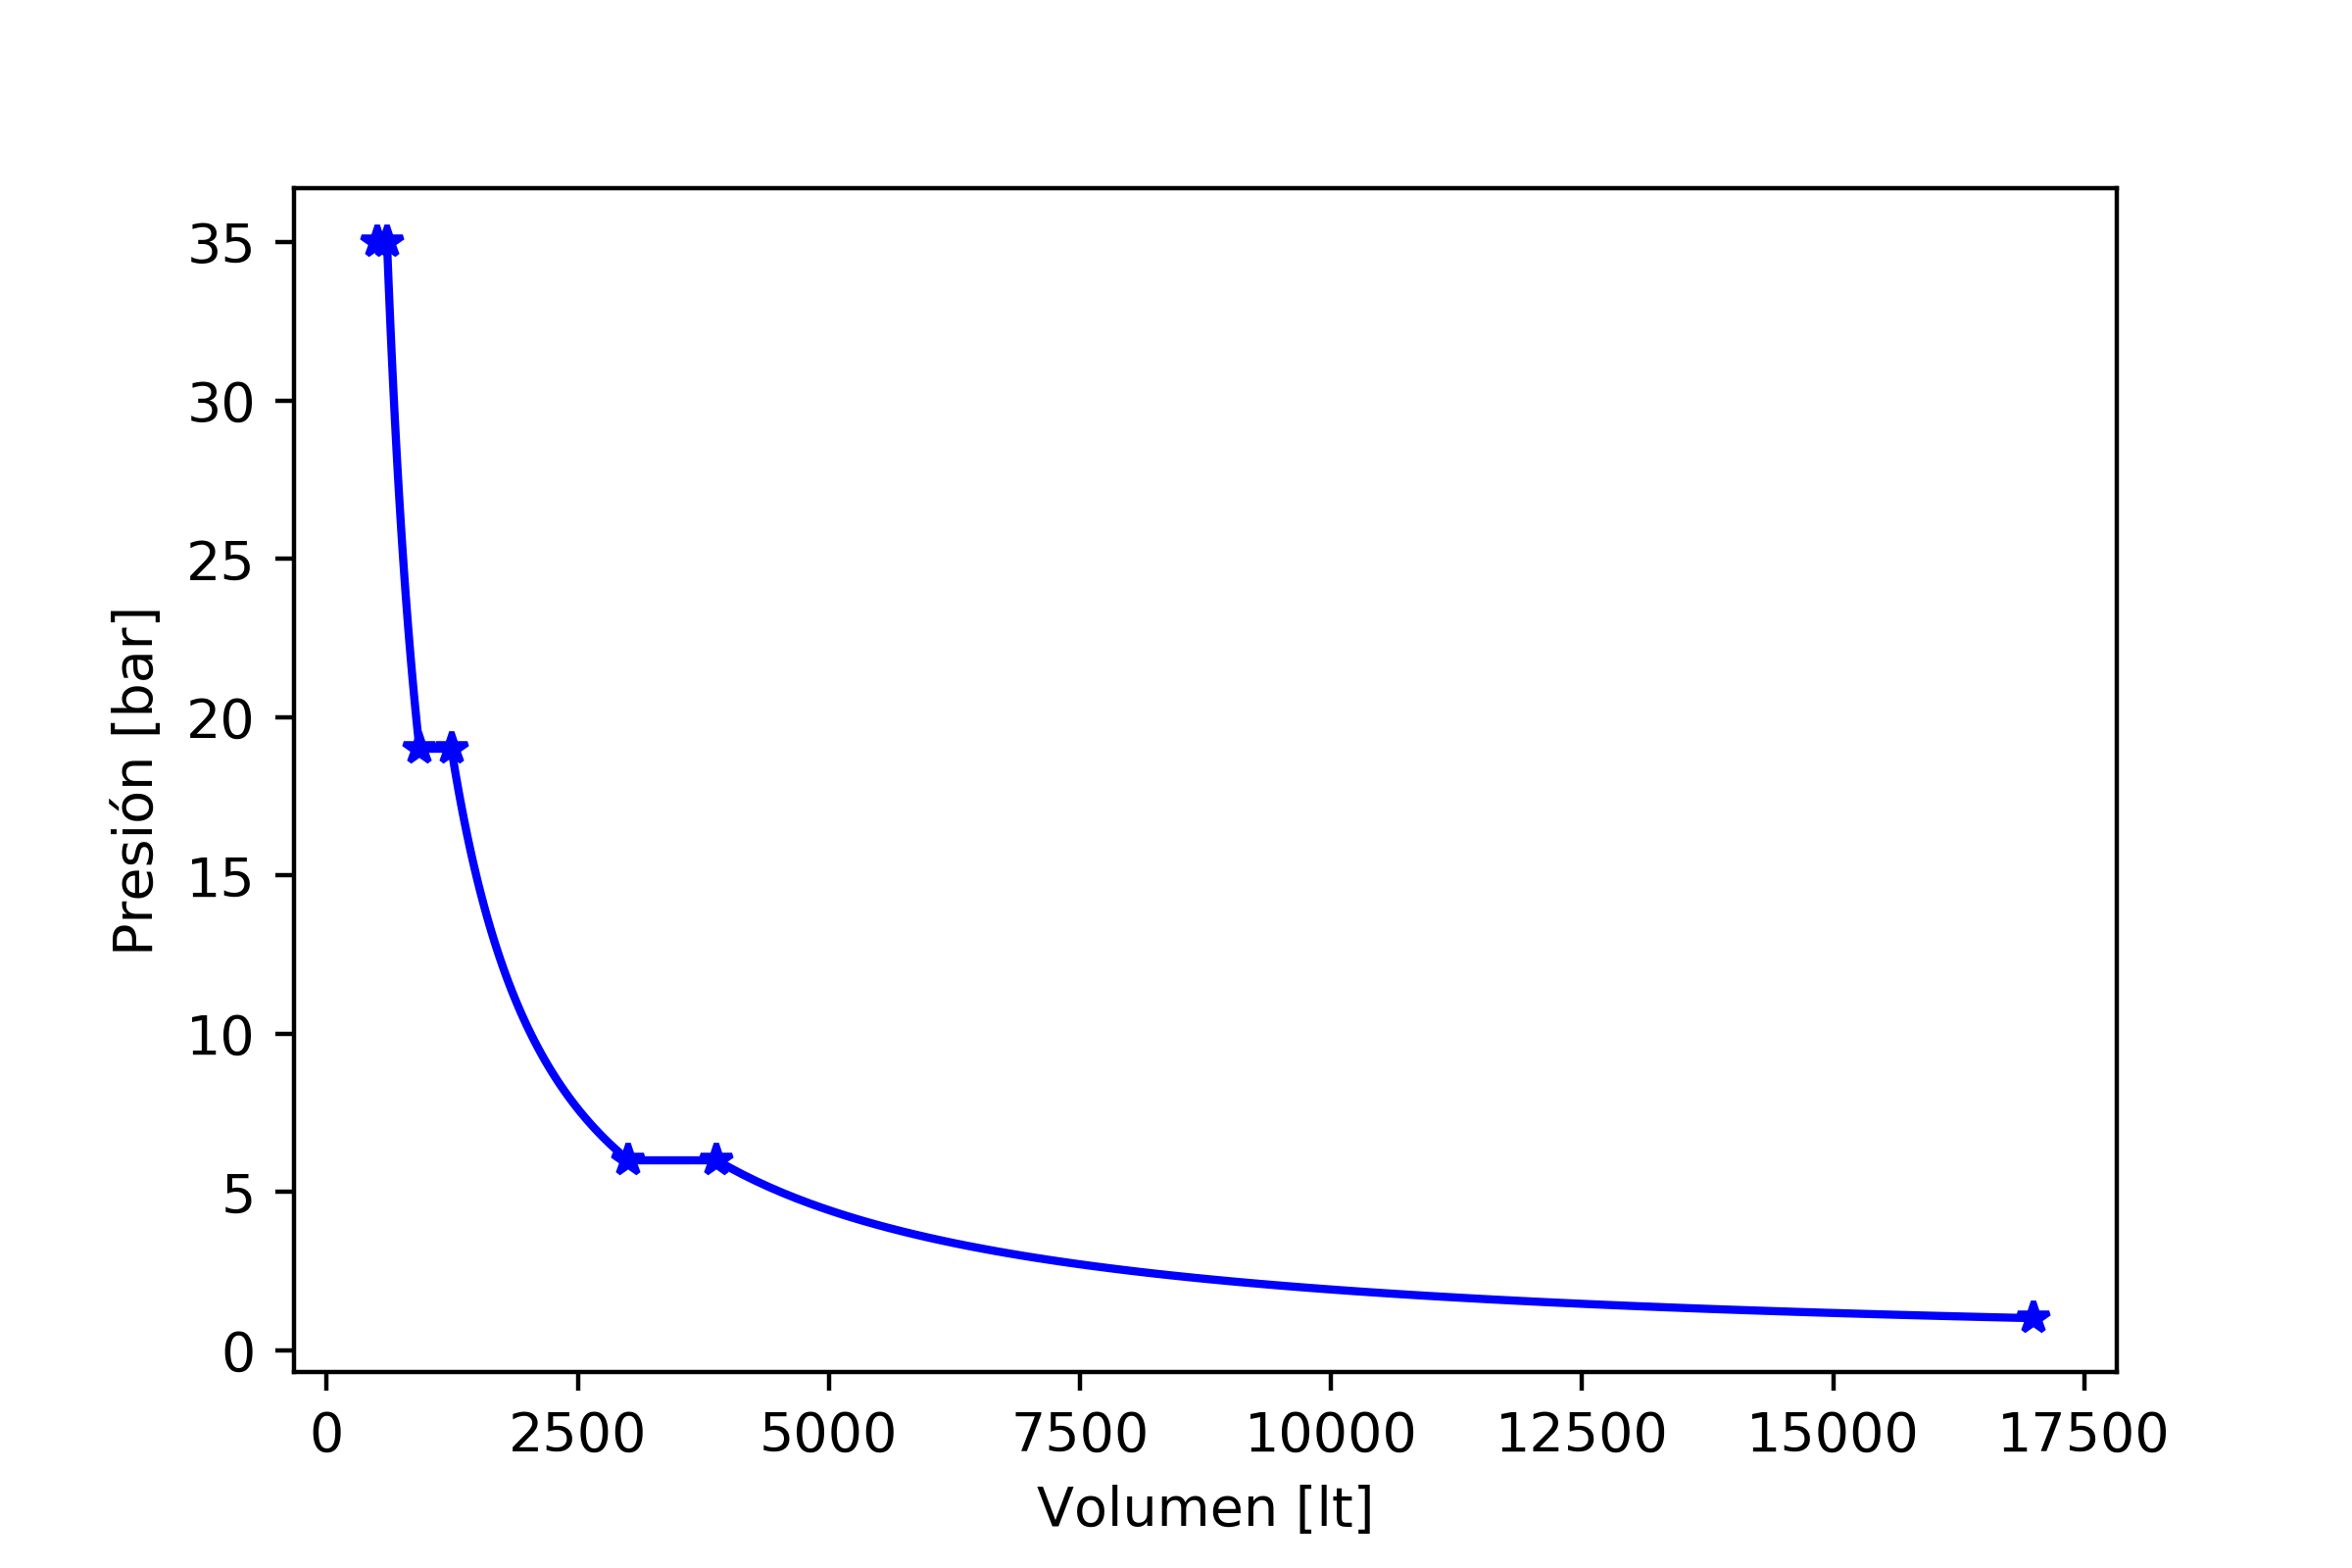
\includegraphics[width = \linewidth]{tiempo33}
\caption{Diagrama PV para un tiempo de 33[min]}
\label{f:t33}
\end{minipage}
\end{figure}

Las figuras presentadas anteriormente tienen su base en las tablas \ref{t:Medidas} a \ref{:Volumen} en donde se presentan los resultados de los cálculos para cada caso. Cabe destacar que las gráficas se realizaron a partir del minuto 12 pues se detectó una mala toma de datos previo a esa medición.





\section{Análisis de resultados}

Las figuras \ref{f:Temperatura} muestra la evolución de la temperatura en el tiempo, en este caso se observa que tanto las temperaturas ambiente $T_0$ como las temperaturas de entrada a los compresores se mantienen relativamente constantes y permanecen en una linea baja de temperaturas inferior a 30$\grados$C a diferencia de las temperaturas de salida que se encuentran en aumento a través del tiempo y a alta temperatura. Esta diferencia entre la entrada y la salida del compresor se debe al calentamiento del gas al interior de los cilindros y el enfriamiento se realiza para disminuir el trabajo necesario para aumentar la presión. En el gráfico se observa una caída o un valle en el minuto 32 que corresponde al momento en que se llega a la presión crítica de la máquina en donde se deja escapar gas y la temperatura disminuye drásticamente para luego retomar el intercambio de calor de estado cuasi estacionario.\\

En cuanto a la evolución de la presión mostrada en el gráfico de la figura \ref{f:Presion} se observa un comportamiento creciente de la presión de escape y la presión del segundo compresor mientras que el primero tiene una presión de descarga más bien baja y casi constante en el tiempo.\\

Los coeficientes politrópicos de la figura \ref{f:Coeficiente} muestran, en las primeras dos etapas de compresión, un comportamiento casi constante salvo por el valle que coincide con el momento del escape por la presión crítica de la máquina. Dado que el coeficiente politrópico es constante y posee baja dispersión a través del tiempo y por tanto, como se vió en el gráfico anterior, a través de la presión de descarga, se puede utilizar con fidelidad para predecir el comportamiento de la máquina en otras puestas en marcha. Esto no sería posible en el caso del tercer compresor pues el coeficiente politrópico posee una dispersión mayor con respecto a un valor fijo.\\

Los gráficos \ref{f:CTiempo} y \ref{f:CPresion} son prácticamente equivalentes pues muestran la evolución del caudal en el tiempo y en contra la presión pero esta última evoluciona crecientemente con el tiempo por lo que resultará una forma similar en ambos casos. En un primer momento llaman la atención unos \textit{peaks} que sobresalen de un comportamiento suave de las curvas, estas irregularidades tienen su origen en la definición teórica del caudal: En la ecuación \ref{e:Caudal} se ve que la función es directamente proporcional al cambio entre una multiplicación de términos, pero como se ha observado en gráficos anteriores, tanto $P_0$, $T_0$ como $T_6$ son prácticamente constantes en el tiempo de modo que el valor del caudal será muy susceptible a cambios bruscos en la presión que es lo que se observa los tiempos 14 y 24 [min] de la figura \ref{f:Presion} en los cuales se observan variaciones bruscas de $P_3$ que generan estas variaciones. La explicación de ellos puede estar en una impresición al tomar las medidas pues las agujas de los manómetros analógicos presentan oscilaciones muy rápidas y, a veces, muy amplias de modo que no es sencillo registrar un valor exacto que describa la masa de aire con fidelidad. Además no se puede fiar del registro que se llevaba antes del minuto 12 pues, como se dijo, los registros estaban errados de modo que no se tiene una visión general y clara del comportamiento del compresor desde la partida hasta su presión crítica. Sin embargo, si se obvian los peaks se observa una leve disminución del caudal del fluido de trabajo a medida que aumenta la presión.\\

En las figuras \ref{f:t14} a \ref{f:t33} se observa la evolución del diagrama \textit{PV} con el tiempo y se aprecia que las presiones de los compresores tienden a estabilizarse a medida que aumenta el tiempo y, como ya se vio en gráficos anteriores, la segunda y tercera etapa tienden a aumentar su presión de descarga. A medida que se aumenta el tiempo (y la presión final de descarga) se observa que la curva se apega más hacia el origen y que se tienen los escalones esperados en un sistema de compresión por etapas los cuales provocan que aumente el rendimiento el compresor en comparación a uno con la misma relación de presiones.

\section{Conclusiones}

Se observó que la presión de descarga final del compresor tiene un comportamiento creciente y que las temperaturas de entrada, luego de los intercambiadores de calor, son prácticamente constantes.\\

Los coeficientes politrópicos de cada etapa pueden servir para caracterizar a la máquina mientras no sean tan dispersos como en el caso de las primeras dos etapas del compresor.\\

Las curvas de caudal, tanto versus la presión como el tiempo, no fueron útiles para realizar deducciones pues los datos previos, desde la partida de la máquina, estaban errados.\\

Se logra obtener el diagrama \textit{PV} del proceso para cualquier tiempo pues la combinación de presiones y temperaturas de cada punto junto con la ley de Avogadro (eq. \ref{e:PavoRaton}) permiten calcular el volumen del gas aún cuando éste no se está midiendo directamente.

\newpage
\section{Anexo}
\setcounter{section}{1}
\renewcommand*\thesection{\Alph{section}}
\begin{table}[H]
\centering
\caption{Medias registradas en la experiencia.}
\label{t:Medidas}
\begin{tabular}{|ccccccccccc|}
\hline
$n$ & $P_1$ {[}Bar{]} & $P_2$ {[}Bar{]} & $P_3$ {[}Bar{]} & $T_0$  {[}$\grados$C{]} & $T_1$  {[}$\grados$C{]} & $T_2$  {[}$\grados$C{]} & $T_3$  {[}$\grados$C{]} & $T_4$  {[}$\grados$C{]} & $T_5$  {[}$\grados$C{]} & $T_6$  {[}$\grados$C{]} \\
\hline \hline
1 & 3.3 & 6 & 4 & 16.2 & 45 & 12 & 40 & 15 & 15 & 15 \\
2 & 3.6 & 6.8 & 5 & 15.7 & 60 & 18 & 49 & 19 & 19 & 12 \\
3 & 3.7 & 7.5 & 6 & 15.3 & 72 & 19 & 51 & 20 & 19 & 13 \\
4 & 3.9 & 8.3 & 7 & 15 & 80 & 18 & 59 & 20 & 20 & 14 \\
5 & 5 & 16 & 24 & 14.8 & 85 & 20 & 62 & 20 & 39 & 16 \\
6 & 5.2 & 17.6 & 27 & 14.7 & 90 & 19 & 85 & 21 & 49 & 18 \\
7 & 5.2 & 17.7 & 28 & 14.6 & 92 & 19 & 92 & 20 & 52 & 18 \\
8 & 5.2 & 17.7 & 28 & 14.5 & 98 & 20 & 99 & 20 & 59 & 19 \\
9 & 5 & 17.5 & 28 & 14.4 & 100 & 20 & 101 & 20 & 58 & 18 \\
10 & 3.7 & 11.9 & 13 & 14.2 & 101 & 20 & 98 & 20 & 49 & 18 \\
11 & 3.8 & 12.1 & 14 & 14.1 & 101 & 21 & 97 & 20 & 45 & 17 \\
12 & 3.9 & 12.6 & 15 & 14.1 & 101 & 21 & 99 & 19 & 46 & 16 \\
13 & 4 & 13 & 16 & 14 & 101 & 20 & 100 & 20 & 49 & 16 \\
14 & 4.1 & 13.4 & 17 & 13.9 & 102 & 21 & 100 & 20 & 50 & 16 \\
15 & 4.3 & 14.6 & 21 & 13.9 & 102 & 21 & 103 & 19 & 52 & 18 \\
16 & 4.3 & 14.9 & 22 & 13.9 & 105 & 21 & 106 & 20 & 56 & 19 \\
17 & 4.4 & 15.1 & 22 & 14 & 107 & 21 & 109 & 19 & 57 & 19 \\
18 & 4.4 & 15.3 & 23 & 14 & 109 & 21 & 110 & 20 & 60 & 19 \\
19 & 4.5 & 15.9 & 24 & 14.1 & 109 & 21 & 111 & 20 & 61 & 19 \\
20 & 4.5 & 15.9 & 24 & 14.1 & 110 & 25 & 112 & 20 & 63 & 19 \\
21 & 4.5 & 16 & 25 & 14.1 & 110 & 25 & 113 & 20 & 63 & 19 \\
22 & 4.5 & 16.2 & 26 & 14.1 & 111 & 22 & 114 & 20 & 65 & 19 \\
23 & 4.6 & 16.8 & 27 & 14.2 & 111 & 22 & 115 & 19 & 67 & 18 \\
24 & 4.6 & 17 & 28 & 14.3 & 111 & 21 & 119 & 19 & 70 & 19 \\
25 & 4.7 & 17.7 & 30 & 14.3 & 112 & 22 & 120 & 19 & 71 & 20 \\
26 & 4.8 & 18 & 31 & 14.3 & 113 & 22 & 121 & 20 & 72 & 20 \\
27 & 4.9 & 18.1 & 32 & 14.3 & 115 & 23 & 121 & 20 & 75 & 20 \\
28 & 4.9 & 18.3 & 33 & 14.4 & 116 & 25 & 122 & 20 & 77 & 20 \\
29 & 5 & 18.6 & 33 & 14.3 & 119 & 25 & 125 & 20 & 79 & 20 \\
30 & 5 & 18.7 & 33.5 & 14.3 & 119 & 25 & 125 & 20 & 79 & 20 \\
31 & 5 & 18.9 & 34 & 14.3 & 119 & 26 & 129 & 20 & 80 & 20 \\
32 & 4.6 & 16.5 & 34.5 & 14.3 & 93 & 24 & 72 & 21 & 54 & 20 \\
33 & 5 & 18 & 34 & 14.3 & 116 & 28 & 121 & 20 & 78 & 19 \\
\hline
\end{tabular}
\end{table}


\begin{table}[H]
\centering
\caption{Coeficientes politrópicos de cada etapa.}
\label{t:Coef}
\begin{tabular}{|ccccc|}
\hline
$n$ & $n_0$ & $n_1$ & $n_2$ & $n_3$ \\
\hline \hline
1 & 0.979109 & 1.04693 & 1.23868 & 1 \\
2 & 0.988713 & 1.07901 & 1.23767 & 1 \\
3 & 0.989601 & 1.10525 & 1.21329 & 1.01795 \\
4 & 0.991888 & 1.12011 & 1.25947 & 1 \\
5 & 1.01452 & 1.11478 & 1.14776 & 1.19466 \\
6 & 1.02388 & 1.12202 & 1.22796 & 1.28605 \\
7 & 1.02653 & 1.12584 & 1.2536 & 1.30934 \\
8 & 1.03326 & 1.13735 & 1.27619 & 1.39826 \\
9 & 1.0323 & 1.14417 & 1.27707 & 1.37231 \\
10 & 1.03037 & 1.17331 & 1.30562 & -6.49658 \\
11 & 1.02468 & 1.17057 & 1.29753 & 2.53051 \\
12 & 1.02528 & 1.16798 & 1.30005 & 2.19485 \\
13 & 1.02822 & 1.16551 & 1.30675 & 1.94658 \\
14 & 1.02878 & 1.1654 & 1.29795 & 1.77618 \\
15 & 1.02898 & 1.16095 & 1.29554 & 1.4525 \\
16 & 1.03271 & 1.16747 & 1.30108 & 1.45766 \\
17 & 1.03375 & 1.16959 & 1.31568 & 1.52223 \\
18 & 1.03634 & 1.17389 & 1.31514 & 1.49439 \\
19 & 1.03686 & 1.17168 & 1.31258 & 1.5027 \\
20 & 1.03887 & 1.17381 & 1.29603 & 1.53795 \\
21 & 1.03838 & 1.17381 & 1.29789 & 1.47568 \\
22 & 1.03987 & 1.17593 & 1.31288 & 1.46389 \\
23 & 1.04134 & 1.17376 & 1.31094 & 1.50603 \\
24 & 1.04374 & 1.17376 & 1.32735 & 1.50959 \\
25 & 1.04377 & 1.17375 & 1.31866 & 1.47986 \\
26 & 1.04427 & 1.17377 & 1.32291 & 1.45649 \\
27 & 1.04658 & 1.17584 & 1.32217 & 1.45905 \\
28 & 1.04795 & 1.17786 & 1.3123 & 1.4576 \\
29 & 1.04973 & 1.18188 & 1.32389 & 1.49942 \\
30 & 1.04952 & 1.18188 & 1.32205 & 1.48681 \\
31 & 1.05019 & 1.18188 & 1.32819 & 1.49244 \\
32 & 1.0268 & 1.13637 & 1.15155 & 1.17703 \\
33 & 1.04842 & 1.17589 & 1.30511 & 1.41978 \\
\hline

\end{tabular}
\end{table}


\begin{table}[H]
\centering
\caption{Volumen en los puntos de medición}
\label{t:volumen}
\begin{tabular}{|ccccccc|}
\hline
n  & $V_0$      & $V_1$      & $V_2$      & $V_3$      & $V_4$      & $V_5$      \\
\hline\hline
1  & 2484.15 & 641.65  & 575.095 & 388.422 & 357.413 & 500     \\
2  & 3005.81 & 761.445 & 665.45  & 434.743 & 394.258 & 512.274 \\
3  & 3488.59 & 897.394 & 759.593 & 466.602 & 421.978 & 510.484 \\
4  & 3968    & 1002.91 & 826.833 & 497.626 & 439.196 & 510.448 \\
5  & 12291.9 & 2576.16 & 2108.62 & 852.057 & 745.28  & 539.772 \\
6  & 13666.8 & 2811.8  & 2262.06 & 925.677 & 760.262 & 553.237 \\
7  & 14149.7 & 2928.21 & 2342.81 & 972.236 & 780.531 & 558.389 \\
8  & 14096.4 & 2966.14 & 2342.78 & 987.482 & 777.86  & 568.458 \\
9  & 14139.9 & 3091.89 & 2429.02 & 1006.96 & 788.963 & 568.693 \\
10 & 6824.75 & 1910.37 & 1496.79 & 691.681 & 546.319 & 553.237 \\
11 & 7334.42 & 2011.08 & 1581.08 & 730.28  & 578.365 & 548.251 \\
12 & 7850    & 2108.64 & 1657.78 & 756.977 & 594.252 & 551.876 \\
13 & 8337.32 & 2195.64 & 1720.3  & 783.391 & 615.439 & 557.064 \\
14 & 8824.29 & 2285.32 & 1791.89 & 806.418 & 633.53  & 558.793 \\
15 & 10709.7 & 2669.21 & 2092.89 & 910.762 & 707.375 & 558.389 \\
16 & 11157.9 & 2803.15 & 2180.47 & 938.413 & 725.56  & 563.324 \\
17 & 11161.8 & 2765.92 & 2140.19 & 934.099 & 714.11  & 565.035 \\
18 & 11646.8 & 2901.29 & 2233.19 & 965.258 & 738.524 & 570.169 \\
19 & 12136.1 & 2967.29 & 2284    & 972.317 & 741.988 & 571.881 \\
20 & 12136.1 & 2975.06 & 2315.06 & 974.848 & 741.988 & 575.304 \\
21 & 12621.2 & 3094    & 2407.61 & 1010.48 & 767.117 & 575.304 \\
22 & 13106.4 & 3221.32 & 2475    & 1039.82 & 787.35  & 578.727 \\
23 & 13643   & 3292.33 & 2529.56 & 1048.27 & 789.004 & 584.149 \\
24 & 14086.6 & 3398.18 & 2602.05 & 1080.99 & 805.331 & 587.284 \\
25 & 15006.3 & 3565.94 & 2732.67 & 1111.31 & 825.817 & 586.986 \\
26 & 15490.1 & 3626.99 & 2772.26 & 1131.92 & 841.867 & 588.692 \\
27 & 15974   & 3696.08 & 2820.03 & 1161.17 & 863.622 & 593.809 \\
28 & 16463.6 & 3817.85 & 2925.07 & 1186.96 & 880.568 & 597.22  \\
29 & 16457.9 & 3783.3  & 2876.43 & 1177.67 & 867.099 & 600.631 \\
30 & 16699.8 & 3838.92 & 2918.71 & 1188.92 & 875.382 & 600.631 \\
31 & 16941.7 & 3894.53 & 2970.93 & 1206.03 & 879.145 & 602.337 \\
32 & 17183.7 & 3951.07 & 3206.5  & 1193.75 & 1017.36 & 557.991 \\
33 & 16999.7 & 3877.97 & 3001.03 & 1242.23 & 923.911 & 600.976 \\
\hline
\end{tabular}
\end{table}

\begin{thebibliography}{x}
	\addcontentsline{toc}{section}{Referencias}
	
	\bibitem{b:Produccion}
W.H. Severns, H.E. Degler \& J.C. Miles. (1961). \textit{La Producción de energía mediante el vapor de agua, el aire y los gases.} New York: REVERTÉ.
	
\end{thebibliography}
\end{document}

